\documentclass[twoside]{book}

% Packages required by doxygen
\usepackage{fixltx2e}
\usepackage{calc}
\usepackage{doxygen}
\usepackage[export]{adjustbox} % also loads graphicx
\usepackage{graphicx}
\usepackage[utf8]{inputenc}
\usepackage{makeidx}
\usepackage{multicol}
\usepackage{multirow}
\PassOptionsToPackage{warn}{textcomp}
\usepackage{textcomp}
\usepackage[nointegrals]{wasysym}
\usepackage[table]{xcolor}

% Font selection
\usepackage[T1]{fontenc}
\usepackage[scaled=.90]{helvet}
\usepackage{courier}
\usepackage{amssymb}
\usepackage{sectsty}
\renewcommand{\familydefault}{\sfdefault}
\allsectionsfont{%
  \fontseries{bc}\selectfont%
  \color{darkgray}%
}
\renewcommand{\DoxyLabelFont}{%
  \fontseries{bc}\selectfont%
  \color{darkgray}%
}
\newcommand{\+}{\discretionary{\mbox{\scriptsize$\hookleftarrow$}}{}{}}

% Page & text layout
\usepackage{geometry}
\geometry{%
  a4paper,%
  top=2.5cm,%
  bottom=2.5cm,%
  left=2.5cm,%
  right=2.5cm%
}
\tolerance=750
\hfuzz=15pt
\hbadness=750
\setlength{\emergencystretch}{15pt}
\setlength{\parindent}{0cm}
\setlength{\parskip}{3ex plus 2ex minus 2ex}
\makeatletter
\renewcommand{\paragraph}{%
  \@startsection{paragraph}{4}{0ex}{-1.0ex}{1.0ex}{%
    \normalfont\normalsize\bfseries\SS@parafont%
  }%
}
\renewcommand{\subparagraph}{%
  \@startsection{subparagraph}{5}{0ex}{-1.0ex}{1.0ex}{%
    \normalfont\normalsize\bfseries\SS@subparafont%
  }%
}
\makeatother

% Headers & footers
\usepackage{fancyhdr}
\pagestyle{fancyplain}
\fancyhead[LE]{\fancyplain{}{\bfseries\thepage}}
\fancyhead[CE]{\fancyplain{}{}}
\fancyhead[RE]{\fancyplain{}{\bfseries\leftmark}}
\fancyhead[LO]{\fancyplain{}{\bfseries\rightmark}}
\fancyhead[CO]{\fancyplain{}{}}
\fancyhead[RO]{\fancyplain{}{\bfseries\thepage}}
\fancyfoot[LE]{\fancyplain{}{}}
\fancyfoot[CE]{\fancyplain{}{}}
\fancyfoot[RE]{\fancyplain{}{\bfseries\scriptsize Generated by Doxygen }}
\fancyfoot[LO]{\fancyplain{}{\bfseries\scriptsize Generated by Doxygen }}
\fancyfoot[CO]{\fancyplain{}{}}
\fancyfoot[RO]{\fancyplain{}{}}
\renewcommand{\footrulewidth}{0.4pt}
\renewcommand{\chaptermark}[1]{%
  \markboth{#1}{}%
}
\renewcommand{\sectionmark}[1]{%
  \markright{\thesection\ #1}%
}

% Indices & bibliography
\usepackage{natbib}
\usepackage[titles]{tocloft}
\setcounter{tocdepth}{3}
\setcounter{secnumdepth}{5}
\makeindex

% Hyperlinks (required, but should be loaded last)
\usepackage{ifpdf}
\ifpdf
  \usepackage[pdftex,pagebackref=true]{hyperref}
\else
  \usepackage[ps2pdf,pagebackref=true]{hyperref}
\fi
\hypersetup{%
  colorlinks=true,%
  linkcolor=blue,%
  citecolor=blue,%
  unicode%
}

% Custom commands
\newcommand{\clearemptydoublepage}{%
  \newpage{\pagestyle{empty}\cleardoublepage}%
}

\usepackage{caption}
\captionsetup{labelsep=space,justification=centering,font={bf},singlelinecheck=off,skip=4pt,position=top}

%===== C O N T E N T S =====

\begin{document}

% Titlepage & ToC
\hypersetup{pageanchor=false,
             bookmarksnumbered=true,
             pdfencoding=unicode
            }
\pagenumbering{alph}
\begin{titlepage}
\vspace*{7cm}
\begin{center}%
{\Large Access Controll Logging Tool \\[1ex]\large V1.\+0.\+3 }\\
\vspace*{1cm}
{\large Generated by Doxygen 1.8.13}\\
\end{center}
\end{titlepage}
\clearemptydoublepage
\pagenumbering{roman}
\tableofcontents
\clearemptydoublepage
\pagenumbering{arabic}
\hypersetup{pageanchor=true}

%--- Begin generated contents ---
\chapter{Assignment 2}
\label{md_README}
\Hypertarget{md_README}
\subsection*{Access Controll Logging Tool}

\subsubsection*{Description}

The access controll logging system monitors and keeps track of every file access and modification that occurs in the system.

\begin{quote}
\+:warning\+:

Systemwide logging can throw errors (notably in the case of \textquotesingle{}gcc\textquotesingle{}) that are not related to the program itself, but to the nature of the temp files these commands use.

\begin{quote}


It is best to disable the preloading before running these commands. \end{quote}
\end{quote}


\subsubsection*{Compilation}

to compile the program, run the following command in the root directory of the project\+:


\begin{DoxyCode}
make clean
make
\end{DoxyCode}


\subsubsection*{Execution}

the program runs in the backround. The systemwide can be enabled and disabled using the following commands\+:


\begin{DoxyCode}
LD\_PRELOAD=./out/libmylib.so    // Enables the logging
LD\_PRELOAD=                     // Disables the logging
\end{DoxyCode}


\subsubsection*{Testing}

The program can be tested with the following commands\+:


\begin{DoxyCode}
make test
\end{DoxyCode}
 
\chapter{Test List}
\label{test}
\Hypertarget{test}

\begin{DoxyRefList}
\item[\label{test__test000005}%
\Hypertarget{test__test000005}%
Global \hyperlink{sarray__test_8c_a9dfb196b1ebe13838bd73446a407155c_a9dfb196b1ebe13838bd73446a407155c}{free\+\_\+test} ()]Test the free function of \hyperlink{}{Misk.\+h}.  
\item[\label{test__test000001}%
\Hypertarget{test__test000001}%
Global \hyperlink{sarray__test_8c_a33f4380cb9acb2659b0a905e8f592207_a33f4380cb9acb2659b0a905e8f592207}{single\+\_\+append\+\_\+test\+\_\+} ()]Test the append function of \hyperlink{}{Misk.\+h}.  
\item[\label{test__test000003}%
\Hypertarget{test__test000003}%
Global \hyperlink{sarray__test_8c_a0ec585a81268a550f110094062a3bb21_a0ec585a81268a550f110094062a3bb21}{single\+\_\+set\+\_\+test} ()]Test the set function of \hyperlink{}{Misk.\+h}.  
\item[\label{test__test000002}%
\Hypertarget{test__test000002}%
Global \hyperlink{sarray__test_8c_a081b7e48daa6ee1b3ee12843ecb33022_a081b7e48daa6ee1b3ee12843ecb33022}{whole\+\_\+append\+\_\+test} ()]Test the append function of \hyperlink{}{Misk.\+h}.  
\item[\label{test__test000004}%
\Hypertarget{test__test000004}%
Global \hyperlink{sarray__test_8c_a58a408c44d40525d202f3db85b83506f_a58a408c44d40525d202f3db85b83506f}{whole\+\_\+set\+\_\+test} ()]Test the set function of \hyperlink{}{Misk.\+h}. 
\end{DoxyRefList}
\chapter{Todo List}
\label{todo}
\Hypertarget{todo}

\begin{DoxyRefList}
\item[\label{todo__todo000002}%
\Hypertarget{todo__todo000002}%
Global \hyperlink{ACL_8c_ae458807f7bf6dc176a3f783da321f6ec_ae458807f7bf6dc176a3f783da321f6ec}{get\+\_\+path} (F\+I\+LE $\ast$f)]test this function 
\end{DoxyRefList}
\chapter{Data Structure Index}
\section{Data Structures}
Here are the data structures with brief descriptions\+:\begin{DoxyCompactList}
\item\contentsline{section}{\hyperlink{structlog__entry}{log\+\_\+entry} }{\pageref{structlog__entry}}{}
\item\contentsline{section}{\hyperlink{structlog__entry__text__hash}{log\+\_\+entry\+\_\+text\+\_\+hash} }{\pageref{structlog__entry__text__hash}}{}
\end{DoxyCompactList}

\chapter{File Index}
\section{File List}
Here is a list of all files with brief descriptions\+:\begin{DoxyCompactList}
\item\contentsline{section}{\hyperlink{ACL_8c}{A\+C\+L.\+c} }{\pageref{ACL_8c}}{}
\item\contentsline{section}{\hyperlink{acmonitor_8c}{acmonitor.\+c} }{\pageref{acmonitor_8c}}{}
\item\contentsline{section}{\hyperlink{fhandler_8c}{fhandler.\+c} }{\pageref{fhandler_8c}}{}
\item\contentsline{section}{\hyperlink{fhandler_8h}{fhandler.\+h} }{\pageref{fhandler_8h}}{}
\item\contentsline{section}{\hyperlink{fmod__test_8c}{fmod\+\_\+test.\+c} }{\pageref{fmod__test_8c}}{}
\item\contentsline{section}{\hyperlink{fperm__test_8c}{fperm\+\_\+test.\+c} }{\pageref{fperm__test_8c}}{}
\item\contentsline{section}{\hyperlink{log_8c}{log.\+c} }{\pageref{log_8c}}{}
\item\contentsline{section}{\hyperlink{log_8h}{log.\+h} }{\pageref{log_8h}}{}
\item\contentsline{section}{\hyperlink{main_8c}{main.\+c} }{\pageref{main_8c}}{}
\item\contentsline{section}{\hyperlink{Misc_8h}{Misc.\+h} }{\pageref{Misc_8h}}{}
\item\contentsline{section}{\hyperlink{sarray__test_8c}{sarray\+\_\+test.\+c} }{\pageref{sarray__test_8c}}{}
\item\contentsline{section}{\hyperlink{template_8c}{template.\+c} }{\pageref{template_8c}}{}
\item\contentsline{section}{\hyperlink{test__aclog_8c}{test\+\_\+aclog.\+c} }{\pageref{test__aclog_8c}}{}
\end{DoxyCompactList}

\chapter{Data Structure Documentation}
\hypertarget{structarray__1d}{}\section{array\+\_\+1d Struct Reference}
\label{structarray__1d}\index{array\+\_\+1d@{array\+\_\+1d}}


A structure to store a 1D array of any type of data.  




{\ttfamily \#include $<$Misc.\+h$>$}

\subsection*{Data Fields}
\begin{DoxyCompactItemize}
\item 
void $\ast$ \hyperlink{structarray__1d_a67bfd60aa42e5469ce9251b4632a6a30_a67bfd60aa42e5469ce9251b4632a6a30}{data}
\item 
int \hyperlink{structarray__1d_acec21fd8404b40eb2b39d5880a6afc45_acec21fd8404b40eb2b39d5880a6afc45}{size}
\end{DoxyCompactItemize}


\subsection{Detailed Description}
A structure to store a 1D array of any type of data. 

\begin{DoxyAttention}{Attention}
The data must typecasted to void$\ast$ before storing. and must be typecasted back to the original type before using. 
\end{DoxyAttention}

\begin{DoxyParams}{Parameters}
{\em data} & A pointer to the array. \\
\hline
{\em size} & The size of the array. \\
\hline
\end{DoxyParams}


\subsection{Field Documentation}
\mbox{\Hypertarget{structarray__1d_a67bfd60aa42e5469ce9251b4632a6a30_a67bfd60aa42e5469ce9251b4632a6a30}\label{structarray__1d_a67bfd60aa42e5469ce9251b4632a6a30_a67bfd60aa42e5469ce9251b4632a6a30}} 
\index{array\+\_\+1d@{array\+\_\+1d}!data@{data}}
\index{data@{data}!array\+\_\+1d@{array\+\_\+1d}}
\subsubsection{\texorpdfstring{data}{data}}
{\footnotesize\ttfamily void$\ast$ array\+\_\+1d\+::data}

\mbox{\Hypertarget{structarray__1d_acec21fd8404b40eb2b39d5880a6afc45_acec21fd8404b40eb2b39d5880a6afc45}\label{structarray__1d_acec21fd8404b40eb2b39d5880a6afc45_acec21fd8404b40eb2b39d5880a6afc45}} 
\index{array\+\_\+1d@{array\+\_\+1d}!size@{size}}
\index{size@{size}!array\+\_\+1d@{array\+\_\+1d}}
\subsubsection{\texorpdfstring{size}{size}}
{\footnotesize\ttfamily int array\+\_\+1d\+::size}



The documentation for this struct was generated from the following file\+:\begin{DoxyCompactItemize}
\item 
\hyperlink{Misc_8h}{Misc.\+h}\end{DoxyCompactItemize}

\hypertarget{structfile__history}{}\section{file\+\_\+history Struct Reference}
\label{structfile__history}\index{file\+\_\+history@{file\+\_\+history}}


File history in the log. Contains logs regarding a file.  




{\ttfamily \#include $<$log.\+h$>$}

\subsection*{Data Fields}
\begin{DoxyCompactItemize}
\item 
char $\ast$ \hyperlink{structfile__history_ab87fc279f8d0a188908e4eadcfafe413_ab87fc279f8d0a188908e4eadcfafe413}{path}
\item 
unsigned int $\ast$ \hyperlink{structfile__history_af68cfa8654b9bff4194c418ac6a2df43_af68cfa8654b9bff4194c418ac6a2df43}{U\+ID}
\item 
unsigned int $\ast$ \hyperlink{structfile__history_a1b25ce4f6b0d07e0eab8382cf9b7519e_a1b25ce4f6b0d07e0eab8382cf9b7519e}{modifications}
\item 
int \hyperlink{structfile__history_a543dae7adc950e19e59aa9e88a658d3b_a543dae7adc950e19e59aa9e88a658d3b}{users}
\end{DoxyCompactItemize}


\subsection{Detailed Description}
File history in the log. Contains logs regarding a file. 


\begin{DoxyParams}{Parameters}
{\em path} & The absolute path of the file. \\
\hline
{\em U\+ID} & The U\+ID of the users that accessed or modified, or attempted to, the file. \\
\hline
{\em modifications} & The number of times the file was modified by each user. \\
\hline
{\em users} & The number of users that modified the file \\
\hline
\end{DoxyParams}


\subsection{Field Documentation}
\mbox{\Hypertarget{structfile__history_a1b25ce4f6b0d07e0eab8382cf9b7519e_a1b25ce4f6b0d07e0eab8382cf9b7519e}\label{structfile__history_a1b25ce4f6b0d07e0eab8382cf9b7519e_a1b25ce4f6b0d07e0eab8382cf9b7519e}} 
\index{file\+\_\+history@{file\+\_\+history}!modifications@{modifications}}
\index{modifications@{modifications}!file\+\_\+history@{file\+\_\+history}}
\subsubsection{\texorpdfstring{modifications}{modifications}}
{\footnotesize\ttfamily unsigned int$\ast$ file\+\_\+history\+::modifications}

\mbox{\Hypertarget{structfile__history_ab87fc279f8d0a188908e4eadcfafe413_ab87fc279f8d0a188908e4eadcfafe413}\label{structfile__history_ab87fc279f8d0a188908e4eadcfafe413_ab87fc279f8d0a188908e4eadcfafe413}} 
\index{file\+\_\+history@{file\+\_\+history}!path@{path}}
\index{path@{path}!file\+\_\+history@{file\+\_\+history}}
\subsubsection{\texorpdfstring{path}{path}}
{\footnotesize\ttfamily char$\ast$ file\+\_\+history\+::path}

\mbox{\Hypertarget{structfile__history_af68cfa8654b9bff4194c418ac6a2df43_af68cfa8654b9bff4194c418ac6a2df43}\label{structfile__history_af68cfa8654b9bff4194c418ac6a2df43_af68cfa8654b9bff4194c418ac6a2df43}} 
\index{file\+\_\+history@{file\+\_\+history}!U\+ID@{U\+ID}}
\index{U\+ID@{U\+ID}!file\+\_\+history@{file\+\_\+history}}
\subsubsection{\texorpdfstring{U\+ID}{UID}}
{\footnotesize\ttfamily unsigned int$\ast$ file\+\_\+history\+::\+U\+ID}

\mbox{\Hypertarget{structfile__history_a543dae7adc950e19e59aa9e88a658d3b_a543dae7adc950e19e59aa9e88a658d3b}\label{structfile__history_a543dae7adc950e19e59aa9e88a658d3b_a543dae7adc950e19e59aa9e88a658d3b}} 
\index{file\+\_\+history@{file\+\_\+history}!users@{users}}
\index{users@{users}!file\+\_\+history@{file\+\_\+history}}
\subsubsection{\texorpdfstring{users}{users}}
{\footnotesize\ttfamily int file\+\_\+history\+::users}



The documentation for this struct was generated from the following file\+:\begin{DoxyCompactItemize}
\item 
\hyperlink{log_8h}{log.\+h}\end{DoxyCompactItemize}

\hypertarget{structlog__entry}{}\section{log\+\_\+entry Struct Reference}
\label{structlog__entry}\index{log\+\_\+entry@{log\+\_\+entry}}


The log entry.  




{\ttfamily \#include $<$log.\+h$>$}

\subsection*{Data Fields}
\begin{DoxyCompactItemize}
\item 
const unsigned int \hyperlink{structlog__entry_a879f3cffed87111c14b5ddca7bf36bfe_a879f3cffed87111c14b5ddca7bf36bfe}{U\+ID}
\item 
const char $\ast$ \hyperlink{structlog__entry_af95c41539cb49570c94f3cdbce83440b_af95c41539cb49570c94f3cdbce83440b}{path}
\item 
const struct tm \hyperlink{structlog__entry_a50022de0184c303275407ebd7eb65c63_a50022de0184c303275407ebd7eb65c63}{timestamp}
\item 
const \hyperlink{log_8h_ab20c54dfb1eb1323b9a3cfe2e6a76270_ab20c54dfb1eb1323b9a3cfe2e6a76270}{access\+\_\+t} \hyperlink{structlog__entry_a36a8d704c97e0fa5f3f83454e2d92662_a36a8d704c97e0fa5f3f83454e2d92662}{access}
\item 
const int \hyperlink{structlog__entry_a7845b16ee2d60f04349b65d55c44dd50_a7845b16ee2d60f04349b65d55c44dd50}{action\+\_\+denied}
\item 
const char \hyperlink{structlog__entry_af2ebb7fded35fda20794591db630571e_af2ebb7fded35fda20794591db630571e}{fingerprint} \mbox{[}33\mbox{]}
\end{DoxyCompactItemize}


\subsection{Detailed Description}
The log entry. 


\begin{DoxyParams}{Parameters}
{\em U\+ID} & The U\+ID of the user. \\
\hline
{\em path} & The absolute path of the file. \\
\hline
{\em timestamp} & The timestamp of the log entry. \\
\hline
{\em access} & The access type. see access\+\_\+t \\
\hline
{\em action\+\_\+denied} & 1 if the action was denied, else 0. \\
\hline
{\em fingerprint} & The fingerprint of the file. \\
\hline
\end{DoxyParams}


\subsection{Field Documentation}
\mbox{\Hypertarget{structlog__entry_a36a8d704c97e0fa5f3f83454e2d92662_a36a8d704c97e0fa5f3f83454e2d92662}\label{structlog__entry_a36a8d704c97e0fa5f3f83454e2d92662_a36a8d704c97e0fa5f3f83454e2d92662}} 
\index{log\+\_\+entry@{log\+\_\+entry}!access@{access}}
\index{access@{access}!log\+\_\+entry@{log\+\_\+entry}}
\subsubsection{\texorpdfstring{access}{access}}
{\footnotesize\ttfamily const \hyperlink{log_8h_ab20c54dfb1eb1323b9a3cfe2e6a76270_ab20c54dfb1eb1323b9a3cfe2e6a76270}{access\+\_\+t} log\+\_\+entry\+::access}

\mbox{\Hypertarget{structlog__entry_a7845b16ee2d60f04349b65d55c44dd50_a7845b16ee2d60f04349b65d55c44dd50}\label{structlog__entry_a7845b16ee2d60f04349b65d55c44dd50_a7845b16ee2d60f04349b65d55c44dd50}} 
\index{log\+\_\+entry@{log\+\_\+entry}!action\+\_\+denied@{action\+\_\+denied}}
\index{action\+\_\+denied@{action\+\_\+denied}!log\+\_\+entry@{log\+\_\+entry}}
\subsubsection{\texorpdfstring{action\+\_\+denied}{action\_denied}}
{\footnotesize\ttfamily const int log\+\_\+entry\+::action\+\_\+denied}

\mbox{\Hypertarget{structlog__entry_af2ebb7fded35fda20794591db630571e_af2ebb7fded35fda20794591db630571e}\label{structlog__entry_af2ebb7fded35fda20794591db630571e_af2ebb7fded35fda20794591db630571e}} 
\index{log\+\_\+entry@{log\+\_\+entry}!fingerprint@{fingerprint}}
\index{fingerprint@{fingerprint}!log\+\_\+entry@{log\+\_\+entry}}
\subsubsection{\texorpdfstring{fingerprint}{fingerprint}}
{\footnotesize\ttfamily const char log\+\_\+entry\+::fingerprint\mbox{[}33\mbox{]}}

\mbox{\Hypertarget{structlog__entry_af95c41539cb49570c94f3cdbce83440b_af95c41539cb49570c94f3cdbce83440b}\label{structlog__entry_af95c41539cb49570c94f3cdbce83440b_af95c41539cb49570c94f3cdbce83440b}} 
\index{log\+\_\+entry@{log\+\_\+entry}!path@{path}}
\index{path@{path}!log\+\_\+entry@{log\+\_\+entry}}
\subsubsection{\texorpdfstring{path}{path}}
{\footnotesize\ttfamily const char$\ast$ log\+\_\+entry\+::path}

\mbox{\Hypertarget{structlog__entry_a50022de0184c303275407ebd7eb65c63_a50022de0184c303275407ebd7eb65c63}\label{structlog__entry_a50022de0184c303275407ebd7eb65c63_a50022de0184c303275407ebd7eb65c63}} 
\index{log\+\_\+entry@{log\+\_\+entry}!timestamp@{timestamp}}
\index{timestamp@{timestamp}!log\+\_\+entry@{log\+\_\+entry}}
\subsubsection{\texorpdfstring{timestamp}{timestamp}}
{\footnotesize\ttfamily const struct tm log\+\_\+entry\+::timestamp}

\mbox{\Hypertarget{structlog__entry_a879f3cffed87111c14b5ddca7bf36bfe_a879f3cffed87111c14b5ddca7bf36bfe}\label{structlog__entry_a879f3cffed87111c14b5ddca7bf36bfe_a879f3cffed87111c14b5ddca7bf36bfe}} 
\index{log\+\_\+entry@{log\+\_\+entry}!U\+ID@{U\+ID}}
\index{U\+ID@{U\+ID}!log\+\_\+entry@{log\+\_\+entry}}
\subsubsection{\texorpdfstring{U\+ID}{UID}}
{\footnotesize\ttfamily const unsigned int log\+\_\+entry\+::\+U\+ID}



The documentation for this struct was generated from the following file\+:\begin{DoxyCompactItemize}
\item 
\hyperlink{log_8h}{log.\+h}\end{DoxyCompactItemize}

\hypertarget{structlog__entry__s}{}\section{log\+\_\+entry\+\_\+s Struct Reference}
\label{structlog__entry__s}\index{log\+\_\+entry\+\_\+s@{log\+\_\+entry\+\_\+s}}


The log entry in strings format.  




{\ttfamily \#include $<$log.\+h$>$}

\subsection*{Data Fields}
\begin{DoxyCompactItemize}
\item 
char \hyperlink{structlog__entry__s_a4cea55f12c34aebb7b3a0a8720e883bf_a4cea55f12c34aebb7b3a0a8720e883bf}{U\+ID} \mbox{[}sizeof(123456789)\mbox{]}
\item 
char \hyperlink{structlog__entry__s_a5af40019a92d555b0317d711b570f14c_a5af40019a92d555b0317d711b570f14c}{path} \mbox{[}256\mbox{]}
\item 
char \hyperlink{structlog__entry__s_ac18d2273a9bf57e659d829e5fff27d70_ac18d2273a9bf57e659d829e5fff27d70}{timestamp} \mbox{[}sizeof(\char`\"{}2024-\/01-\/01 00\+:00\+:00\char`\"{})\mbox{]}
\item 
char \hyperlink{structlog__entry__s_afd6b8cbb3e041417f504dd9b7653d43a_afd6b8cbb3e041417f504dd9b7653d43a}{access} \mbox{[}6\mbox{]}
\item 
char \hyperlink{structlog__entry__s_aab4fe84d4d2bd2f0122dca8a4362a53f_aab4fe84d4d2bd2f0122dca8a4362a53f}{action\+\_\+denied} \mbox{[}1\mbox{]}
\item 
char \hyperlink{structlog__entry__s_adcc31a7a6fb6279625c938bde82d4310_adcc31a7a6fb6279625c938bde82d4310}{fingerprint} \mbox{[}33\mbox{]}
\end{DoxyCompactItemize}


\subsection{Detailed Description}
The log entry in strings format. 


\begin{DoxyParams}{Parameters}
{\em U\+ID} & The U\+ID of the user. \\
\hline
{\em path} & The absolute path of the file. \\
\hline
{\em timestamp} & The timestamp of the log entry. \\
\hline
{\em access} & The access type. see access\+\_\+t \\
\hline
{\em action\+\_\+denied} & 1 if the action was denied, else 0. \\
\hline
{\em fingerprint} & The fingerprint of the file. \\
\hline
\end{DoxyParams}


\subsection{Field Documentation}
\mbox{\Hypertarget{structlog__entry__s_afd6b8cbb3e041417f504dd9b7653d43a_afd6b8cbb3e041417f504dd9b7653d43a}\label{structlog__entry__s_afd6b8cbb3e041417f504dd9b7653d43a_afd6b8cbb3e041417f504dd9b7653d43a}} 
\index{log\+\_\+entry\+\_\+s@{log\+\_\+entry\+\_\+s}!access@{access}}
\index{access@{access}!log\+\_\+entry\+\_\+s@{log\+\_\+entry\+\_\+s}}
\subsubsection{\texorpdfstring{access}{access}}
{\footnotesize\ttfamily char log\+\_\+entry\+\_\+s\+::access\mbox{[}6\mbox{]}}

\mbox{\Hypertarget{structlog__entry__s_aab4fe84d4d2bd2f0122dca8a4362a53f_aab4fe84d4d2bd2f0122dca8a4362a53f}\label{structlog__entry__s_aab4fe84d4d2bd2f0122dca8a4362a53f_aab4fe84d4d2bd2f0122dca8a4362a53f}} 
\index{log\+\_\+entry\+\_\+s@{log\+\_\+entry\+\_\+s}!action\+\_\+denied@{action\+\_\+denied}}
\index{action\+\_\+denied@{action\+\_\+denied}!log\+\_\+entry\+\_\+s@{log\+\_\+entry\+\_\+s}}
\subsubsection{\texorpdfstring{action\+\_\+denied}{action\_denied}}
{\footnotesize\ttfamily char log\+\_\+entry\+\_\+s\+::action\+\_\+denied\mbox{[}1\mbox{]}}

\mbox{\Hypertarget{structlog__entry__s_adcc31a7a6fb6279625c938bde82d4310_adcc31a7a6fb6279625c938bde82d4310}\label{structlog__entry__s_adcc31a7a6fb6279625c938bde82d4310_adcc31a7a6fb6279625c938bde82d4310}} 
\index{log\+\_\+entry\+\_\+s@{log\+\_\+entry\+\_\+s}!fingerprint@{fingerprint}}
\index{fingerprint@{fingerprint}!log\+\_\+entry\+\_\+s@{log\+\_\+entry\+\_\+s}}
\subsubsection{\texorpdfstring{fingerprint}{fingerprint}}
{\footnotesize\ttfamily char log\+\_\+entry\+\_\+s\+::fingerprint\mbox{[}33\mbox{]}}

\mbox{\Hypertarget{structlog__entry__s_a5af40019a92d555b0317d711b570f14c_a5af40019a92d555b0317d711b570f14c}\label{structlog__entry__s_a5af40019a92d555b0317d711b570f14c_a5af40019a92d555b0317d711b570f14c}} 
\index{log\+\_\+entry\+\_\+s@{log\+\_\+entry\+\_\+s}!path@{path}}
\index{path@{path}!log\+\_\+entry\+\_\+s@{log\+\_\+entry\+\_\+s}}
\subsubsection{\texorpdfstring{path}{path}}
{\footnotesize\ttfamily char log\+\_\+entry\+\_\+s\+::path\mbox{[}256\mbox{]}}

\mbox{\Hypertarget{structlog__entry__s_ac18d2273a9bf57e659d829e5fff27d70_ac18d2273a9bf57e659d829e5fff27d70}\label{structlog__entry__s_ac18d2273a9bf57e659d829e5fff27d70_ac18d2273a9bf57e659d829e5fff27d70}} 
\index{log\+\_\+entry\+\_\+s@{log\+\_\+entry\+\_\+s}!timestamp@{timestamp}}
\index{timestamp@{timestamp}!log\+\_\+entry\+\_\+s@{log\+\_\+entry\+\_\+s}}
\subsubsection{\texorpdfstring{timestamp}{timestamp}}
{\footnotesize\ttfamily char log\+\_\+entry\+\_\+s\+::timestamp\mbox{[}sizeof(\char`\"{}2024-\/01-\/01 00\+:00\+:00\char`\"{})\mbox{]}}

\mbox{\Hypertarget{structlog__entry__s_a4cea55f12c34aebb7b3a0a8720e883bf_a4cea55f12c34aebb7b3a0a8720e883bf}\label{structlog__entry__s_a4cea55f12c34aebb7b3a0a8720e883bf_a4cea55f12c34aebb7b3a0a8720e883bf}} 
\index{log\+\_\+entry\+\_\+s@{log\+\_\+entry\+\_\+s}!U\+ID@{U\+ID}}
\index{U\+ID@{U\+ID}!log\+\_\+entry\+\_\+s@{log\+\_\+entry\+\_\+s}}
\subsubsection{\texorpdfstring{U\+ID}{UID}}
{\footnotesize\ttfamily char log\+\_\+entry\+\_\+s\+::\+U\+ID\mbox{[}sizeof(123456789)\mbox{]}}



The documentation for this struct was generated from the following file\+:\begin{DoxyCompactItemize}
\item 
\hyperlink{log_8h}{log.\+h}\end{DoxyCompactItemize}

\hypertarget{structString__array}{}\section{String\+\_\+array Struct Reference}
\label{structString__array}\index{String\+\_\+array@{String\+\_\+array}}


A structure to store an array of strings.  




{\ttfamily \#include $<$Misc.\+h$>$}

\subsection*{Data Fields}
\begin{DoxyCompactItemize}
\item 
char $\ast$$\ast$ \hyperlink{structString__array_afbe749a8998c54158933158ebc48dce9_afbe749a8998c54158933158ebc48dce9}{data}
\item 
size\+\_\+t \hyperlink{structString__array_afe557fc0c5136ee70c765ba49513c098_afe557fc0c5136ee70c765ba49513c098}{size}
\item 
size\+\_\+t \hyperlink{structString__array_a6c31358160c33bad3f63da0b677bec82_a6c31358160c33bad3f63da0b677bec82}{capacity}
\item 
size\+\_\+t \hyperlink{structString__array_a9acda89272e9c00036c20f0643aa81e1_a9acda89272e9c00036c20f0643aa81e1}{data\+\_\+size}
\end{DoxyCompactItemize}


\subsection{Detailed Description}
A structure to store an array of strings. 


\begin{DoxyParams}{Parameters}
{\em data} & A pointer to the array of strings. \\
\hline
{\em size} & The size of the array. \\
\hline
{\em capacity} & The capacity of the array. \\
\hline
{\em data\+\_\+size} & The size for each string in the array. \\
\hline
\end{DoxyParams}


\subsection{Field Documentation}
\mbox{\Hypertarget{structString__array_a6c31358160c33bad3f63da0b677bec82_a6c31358160c33bad3f63da0b677bec82}\label{structString__array_a6c31358160c33bad3f63da0b677bec82_a6c31358160c33bad3f63da0b677bec82}} 
\index{String\+\_\+array@{String\+\_\+array}!capacity@{capacity}}
\index{capacity@{capacity}!String\+\_\+array@{String\+\_\+array}}
\subsubsection{\texorpdfstring{capacity}{capacity}}
{\footnotesize\ttfamily size\+\_\+t String\+\_\+array\+::capacity}

\mbox{\Hypertarget{structString__array_afbe749a8998c54158933158ebc48dce9_afbe749a8998c54158933158ebc48dce9}\label{structString__array_afbe749a8998c54158933158ebc48dce9_afbe749a8998c54158933158ebc48dce9}} 
\index{String\+\_\+array@{String\+\_\+array}!data@{data}}
\index{data@{data}!String\+\_\+array@{String\+\_\+array}}
\subsubsection{\texorpdfstring{data}{data}}
{\footnotesize\ttfamily char$\ast$$\ast$ String\+\_\+array\+::data}

\mbox{\Hypertarget{structString__array_a9acda89272e9c00036c20f0643aa81e1_a9acda89272e9c00036c20f0643aa81e1}\label{structString__array_a9acda89272e9c00036c20f0643aa81e1_a9acda89272e9c00036c20f0643aa81e1}} 
\index{String\+\_\+array@{String\+\_\+array}!data\+\_\+size@{data\+\_\+size}}
\index{data\+\_\+size@{data\+\_\+size}!String\+\_\+array@{String\+\_\+array}}
\subsubsection{\texorpdfstring{data\+\_\+size}{data\_size}}
{\footnotesize\ttfamily size\+\_\+t String\+\_\+array\+::data\+\_\+size}

\mbox{\Hypertarget{structString__array_afe557fc0c5136ee70c765ba49513c098_afe557fc0c5136ee70c765ba49513c098}\label{structString__array_afe557fc0c5136ee70c765ba49513c098_afe557fc0c5136ee70c765ba49513c098}} 
\index{String\+\_\+array@{String\+\_\+array}!size@{size}}
\index{size@{size}!String\+\_\+array@{String\+\_\+array}}
\subsubsection{\texorpdfstring{size}{size}}
{\footnotesize\ttfamily size\+\_\+t String\+\_\+array\+::size}



The documentation for this struct was generated from the following file\+:\begin{DoxyCompactItemize}
\item 
\hyperlink{Misc_8h}{Misc.\+h}\end{DoxyCompactItemize}

\hypertarget{structuser__history}{}\section{user\+\_\+history Struct Reference}
\label{structuser__history}\index{user\+\_\+history@{user\+\_\+history}}


User history in the log. Contains all files the user attempted ro access or modify but was rejected.  




{\ttfamily \#include $<$log.\+h$>$}

\subsection*{Data Fields}
\begin{DoxyCompactItemize}
\item 
unsigned int \hyperlink{structuser__history_ac06f0a0d7274aa206bda3dde0e8e8a9e_ac06f0a0d7274aa206bda3dde0e8e8a9e}{U\+ID}
\item 
int \hyperlink{structuser__history_ad90b0ce88a6a7ca1b89a3266c9f961f6_ad90b0ce88a6a7ca1b89a3266c9f961f6}{strikes}
\item 
char $\ast$$\ast$ \hyperlink{structuser__history_a668329217bf805a1f95c20925598f32d_a668329217bf805a1f95c20925598f32d}{path}
\end{DoxyCompactItemize}


\subsection{Detailed Description}
User history in the log. Contains all files the user attempted ro access or modify but was rejected. 


\begin{DoxyParams}{Parameters}
{\em U\+ID} & The U\+ID of the user. \\
\hline
{\em strikes} & The number of strikes the user has. \\
\hline
{\em path} & The absolute path of the files accessed or modified. \\
\hline
\end{DoxyParams}


\subsection{Field Documentation}
\mbox{\Hypertarget{structuser__history_a668329217bf805a1f95c20925598f32d_a668329217bf805a1f95c20925598f32d}\label{structuser__history_a668329217bf805a1f95c20925598f32d_a668329217bf805a1f95c20925598f32d}} 
\index{user\+\_\+history@{user\+\_\+history}!path@{path}}
\index{path@{path}!user\+\_\+history@{user\+\_\+history}}
\subsubsection{\texorpdfstring{path}{path}}
{\footnotesize\ttfamily char$\ast$$\ast$ user\+\_\+history\+::path}

\mbox{\Hypertarget{structuser__history_ad90b0ce88a6a7ca1b89a3266c9f961f6_ad90b0ce88a6a7ca1b89a3266c9f961f6}\label{structuser__history_ad90b0ce88a6a7ca1b89a3266c9f961f6_ad90b0ce88a6a7ca1b89a3266c9f961f6}} 
\index{user\+\_\+history@{user\+\_\+history}!strikes@{strikes}}
\index{strikes@{strikes}!user\+\_\+history@{user\+\_\+history}}
\subsubsection{\texorpdfstring{strikes}{strikes}}
{\footnotesize\ttfamily int user\+\_\+history\+::strikes}

\mbox{\Hypertarget{structuser__history_ac06f0a0d7274aa206bda3dde0e8e8a9e_ac06f0a0d7274aa206bda3dde0e8e8a9e}\label{structuser__history_ac06f0a0d7274aa206bda3dde0e8e8a9e_ac06f0a0d7274aa206bda3dde0e8e8a9e}} 
\index{user\+\_\+history@{user\+\_\+history}!U\+ID@{U\+ID}}
\index{U\+ID@{U\+ID}!user\+\_\+history@{user\+\_\+history}}
\subsubsection{\texorpdfstring{U\+ID}{UID}}
{\footnotesize\ttfamily unsigned int user\+\_\+history\+::\+U\+ID}



The documentation for this struct was generated from the following file\+:\begin{DoxyCompactItemize}
\item 
\hyperlink{log_8h}{log.\+h}\end{DoxyCompactItemize}

\chapter{File Documentation}
\hypertarget{ACL_8c}{}\section{A\+C\+L.\+c File Reference}
\label{ACL_8c}\index{A\+C\+L.\+c@{A\+C\+L.\+c}}
{\ttfamily \#include $<$stdio.\+h$>$}\newline
{\ttfamily \#include $<$stdlib.\+h$>$}\newline
{\ttfamily \#include $<$string.\+h$>$}\newline
{\ttfamily \#include $<$dlfcn.\+h$>$}\newline
{\ttfamily \#include $<$errno.\+h$>$}\newline
{\ttfamily \#include $<$unistd.\+h$>$}\newline
{\ttfamily \#include $<$stdarg.\+h$>$}\newline
{\ttfamily \#include $<$openssl/md5.\+h$>$}\newline
{\ttfamily \#include \char`\"{}log.\+h\char`\"{}}\newline
{\ttfamily \#include \char`\"{}fhandler.\+h\char`\"{}}\newline
Include dependency graph for A\+C\+L.\+c\+:\nopagebreak
\begin{figure}[H]
\begin{center}
\leavevmode
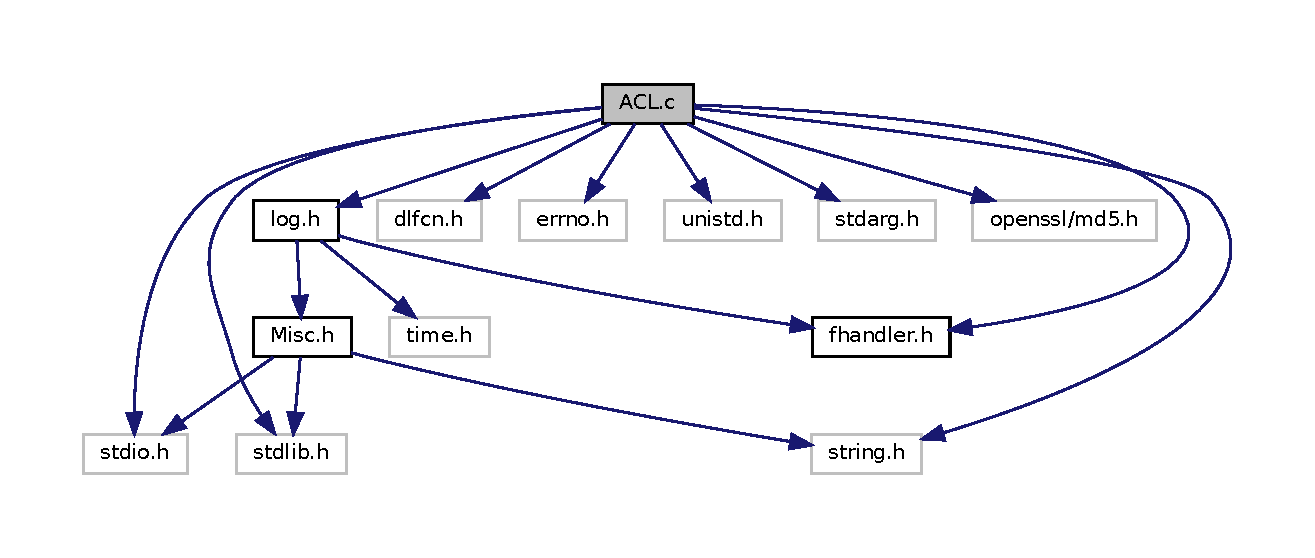
\includegraphics[width=350pt]{ACL_8c__incl}
\end{center}
\end{figure}
\subsection*{Macros}
\begin{DoxyCompactItemize}
\item 
\#define \hyperlink{ACL_8c_a369266c24eacffb87046522897a570d5_a369266c24eacffb87046522897a570d5}{\+\_\+\+G\+N\+U\+\_\+\+S\+O\+U\+R\+CE}
\item 
\#define \hyperlink{ACL_8c_ac4c027058e9ccd1d4dce6a718af0b422_ac4c027058e9ccd1d4dce6a718af0b422}{printd}(format, ...)
\item 
\#define \hyperlink{ACL_8c_a8b3a3c4c8735fffe0d3b0ab6c7053667_a8b3a3c4c8735fffe0d3b0ab6c7053667}{printld}(format, ...)
\item 
\#define \hyperlink{ACL_8c_a483d4c865c4cb956ffe919f48867641a_a483d4c865c4cb956ffe919f48867641a}{printv}(format, ...)
\end{DoxyCompactItemize}
\subsection*{Functions}
\begin{DoxyCompactItemize}
\item 
char $\ast$ \hyperlink{ACL_8c_ae458807f7bf6dc176a3f783da321f6ec_ae458807f7bf6dc176a3f783da321f6ec}{get\+\_\+path} (F\+I\+LE $\ast$f)
\begin{DoxyCompactList}\small\item\em returns the absolute path of a file stream \end{DoxyCompactList}\item 
unsigned char $\ast$ \hyperlink{ACL_8c_a7da6115f144b2d630d5f090399ee4645_a7da6115f144b2d630d5f090399ee4645}{Hash} (F\+I\+LE $\ast$fp)
\begin{DoxyCompactList}\small\item\em Creates a hash key from the contents of a file. \end{DoxyCompactList}\item 
unsigned char $\ast$ \hyperlink{ACL_8c_a4c27f974a9c92361a21efd1bb444e170_a4c27f974a9c92361a21efd1bb444e170}{Hash\+\_\+string} (char $\ast$str)
\begin{DoxyCompactList}\small\item\em Creates a hash key from a string. \end{DoxyCompactList}\end{DoxyCompactItemize}


\subsection{Macro Definition Documentation}
\mbox{\Hypertarget{ACL_8c_a369266c24eacffb87046522897a570d5_a369266c24eacffb87046522897a570d5}\label{ACL_8c_a369266c24eacffb87046522897a570d5_a369266c24eacffb87046522897a570d5}} 
\index{A\+C\+L.\+c@{A\+C\+L.\+c}!\+\_\+\+G\+N\+U\+\_\+\+S\+O\+U\+R\+CE@{\+\_\+\+G\+N\+U\+\_\+\+S\+O\+U\+R\+CE}}
\index{\+\_\+\+G\+N\+U\+\_\+\+S\+O\+U\+R\+CE@{\+\_\+\+G\+N\+U\+\_\+\+S\+O\+U\+R\+CE}!A\+C\+L.\+c@{A\+C\+L.\+c}}
\subsubsection{\texorpdfstring{\+\_\+\+G\+N\+U\+\_\+\+S\+O\+U\+R\+CE}{\_GNU\_SOURCE}}
{\footnotesize\ttfamily \#define \+\_\+\+G\+N\+U\+\_\+\+S\+O\+U\+R\+CE}

\mbox{\Hypertarget{ACL_8c_ac4c027058e9ccd1d4dce6a718af0b422_ac4c027058e9ccd1d4dce6a718af0b422}\label{ACL_8c_ac4c027058e9ccd1d4dce6a718af0b422_ac4c027058e9ccd1d4dce6a718af0b422}} 
\index{A\+C\+L.\+c@{A\+C\+L.\+c}!printd@{printd}}
\index{printd@{printd}!A\+C\+L.\+c@{A\+C\+L.\+c}}
\subsubsection{\texorpdfstring{printd}{printd}}
{\footnotesize\ttfamily \#define printd(\begin{DoxyParamCaption}\item[{}]{format,  }\item[{}]{... }\end{DoxyParamCaption})}

\mbox{\Hypertarget{ACL_8c_a8b3a3c4c8735fffe0d3b0ab6c7053667_a8b3a3c4c8735fffe0d3b0ab6c7053667}\label{ACL_8c_a8b3a3c4c8735fffe0d3b0ab6c7053667_a8b3a3c4c8735fffe0d3b0ab6c7053667}} 
\index{A\+C\+L.\+c@{A\+C\+L.\+c}!printld@{printld}}
\index{printld@{printld}!A\+C\+L.\+c@{A\+C\+L.\+c}}
\subsubsection{\texorpdfstring{printld}{printld}}
{\footnotesize\ttfamily \#define printld(\begin{DoxyParamCaption}\item[{}]{format,  }\item[{}]{... }\end{DoxyParamCaption})}

\mbox{\Hypertarget{ACL_8c_a483d4c865c4cb956ffe919f48867641a_a483d4c865c4cb956ffe919f48867641a}\label{ACL_8c_a483d4c865c4cb956ffe919f48867641a_a483d4c865c4cb956ffe919f48867641a}} 
\index{A\+C\+L.\+c@{A\+C\+L.\+c}!printv@{printv}}
\index{printv@{printv}!A\+C\+L.\+c@{A\+C\+L.\+c}}
\subsubsection{\texorpdfstring{printv}{printv}}
{\footnotesize\ttfamily \#define printv(\begin{DoxyParamCaption}\item[{}]{format,  }\item[{}]{... }\end{DoxyParamCaption})}



\subsection{Function Documentation}
\mbox{\Hypertarget{ACL_8c_ae458807f7bf6dc176a3f783da321f6ec_ae458807f7bf6dc176a3f783da321f6ec}\label{ACL_8c_ae458807f7bf6dc176a3f783da321f6ec_ae458807f7bf6dc176a3f783da321f6ec}} 
\index{A\+C\+L.\+c@{A\+C\+L.\+c}!get\+\_\+path@{get\+\_\+path}}
\index{get\+\_\+path@{get\+\_\+path}!A\+C\+L.\+c@{A\+C\+L.\+c}}
\subsubsection{\texorpdfstring{get\+\_\+path()}{get\_path()}}
{\footnotesize\ttfamily char$\ast$ get\+\_\+path (\begin{DoxyParamCaption}\item[{F\+I\+LE $\ast$}]{f }\end{DoxyParamCaption})}



returns the absolute path of a file stream 


\begin{DoxyParams}{Parameters}
{\em f} & The file stream \\
\hline
\end{DoxyParams}
\begin{DoxyReturn}{Returns}
char$\ast$ The absolute path of the file stream
\end{DoxyReturn}
\begin{DoxyWarning}{Warning}
This function is not tested.
\end{DoxyWarning}
\begin{DoxyRefDesc}{Todo}
\item[\hyperlink{todo__todo000002}{Todo}]test this function \end{DoxyRefDesc}
\mbox{\Hypertarget{ACL_8c_a7da6115f144b2d630d5f090399ee4645_a7da6115f144b2d630d5f090399ee4645}\label{ACL_8c_a7da6115f144b2d630d5f090399ee4645_a7da6115f144b2d630d5f090399ee4645}} 
\index{A\+C\+L.\+c@{A\+C\+L.\+c}!Hash@{Hash}}
\index{Hash@{Hash}!A\+C\+L.\+c@{A\+C\+L.\+c}}
\subsubsection{\texorpdfstring{Hash()}{Hash()}}
{\footnotesize\ttfamily unsigned char$\ast$ Hash (\begin{DoxyParamCaption}\item[{F\+I\+LE $\ast$}]{fp }\end{DoxyParamCaption})}



Creates a hash key from the contents of a file. 


\begin{DoxyParams}{Parameters}
{\em fp} & The file stream \\
\hline
\end{DoxyParams}
\begin{DoxyReturn}{Returns}
unsigned char$\ast$ The hash key 
\end{DoxyReturn}
\mbox{\Hypertarget{ACL_8c_a4c27f974a9c92361a21efd1bb444e170_a4c27f974a9c92361a21efd1bb444e170}\label{ACL_8c_a4c27f974a9c92361a21efd1bb444e170_a4c27f974a9c92361a21efd1bb444e170}} 
\index{A\+C\+L.\+c@{A\+C\+L.\+c}!Hash\+\_\+string@{Hash\+\_\+string}}
\index{Hash\+\_\+string@{Hash\+\_\+string}!A\+C\+L.\+c@{A\+C\+L.\+c}}
\subsubsection{\texorpdfstring{Hash\+\_\+string()}{Hash\_string()}}
{\footnotesize\ttfamily unsigned char$\ast$ Hash\+\_\+string (\begin{DoxyParamCaption}\item[{char $\ast$}]{str }\end{DoxyParamCaption})}



Creates a hash key from a string. 


\begin{DoxyParams}{Parameters}
{\em str} & The string \\
\hline
\end{DoxyParams}
\begin{DoxyReturn}{Returns}
unsigned char$\ast$ The hash key 
\end{DoxyReturn}

\hypertarget{acmonitor_8c}{}\section{acmonitor.\+c File Reference}
\label{acmonitor_8c}\index{acmonitor.\+c@{acmonitor.\+c}}
{\ttfamily \#include \char`\"{}lib/log.\+h\char`\"{}}\newline
{\ttfamily \#include \char`\"{}lib/fhandler.\+h\char`\"{}}\newline
{\ttfamily \#include $<$stdio.\+h$>$}\newline
{\ttfamily \#include $<$stdlib.\+h$>$}\newline
{\ttfamily \#include $<$string.\+h$>$}\newline
Include dependency graph for acmonitor.\+c\+:
\nopagebreak
\begin{figure}[H]
\begin{center}
\leavevmode
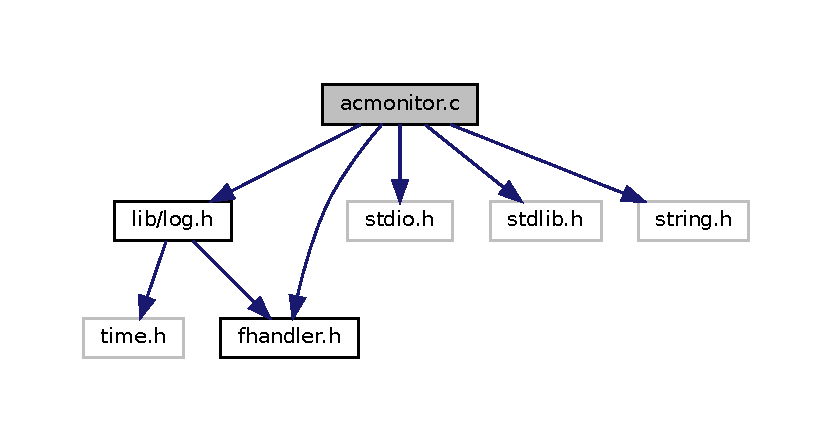
\includegraphics[width=350pt]{acmonitor_8c__incl}
\end{center}
\end{figure}
\subsection*{Data Structures}
\begin{DoxyCompactItemize}
\item 
struct \hyperlink{structlog__entry__text__hash}{log\+\_\+entry\+\_\+text\+\_\+hash}
\end{DoxyCompactItemize}
\subsection*{Macros}
\begin{DoxyCompactItemize}
\item 
\#define \hyperlink{acmonitor_8c_aff6732b7d46ac296a7b8d61ada41d949_aff6732b7d46ac296a7b8d61ada41d949}{\+\_\+\+L\+O\+G\+\_\+\+B\+U\+F\+F\+E\+R\+\_\+\+S\+I\+Z\+E\+\_\+}~1024
\item 
\#define \hyperlink{acmonitor_8c_a73708c27921af699a08573001ea2584d_a73708c27921af699a08573001ea2584d}{\+\_\+\+M\+A\+X\+\_\+\+S\+T\+R\+I\+K\+E\+\_\+}~7
\end{DoxyCompactItemize}
\subsection*{Typedefs}
\begin{DoxyCompactItemize}
\item 
typedef struct \hyperlink{structlog__entry__text__hash}{log\+\_\+entry\+\_\+text\+\_\+hash} \hyperlink{acmonitor_8c_a2c07adb053c6cb67f66231ae9cc7734d_a2c07adb053c6cb67f66231ae9cc7734d}{logf\+\_\+t}
\end{DoxyCompactItemize}
\subsection*{Functions}
\begin{DoxyCompactItemize}
\item 
\hyperlink{acmonitor_8c_a2c07adb053c6cb67f66231ae9cc7734d_a2c07adb053c6cb67f66231ae9cc7734d}{logf\+\_\+t} \hyperlink{acmonitor_8c_a88ee5df83d5ccb61194f75e95db7771b_a88ee5df83d5ccb61194f75e95db7771b}{parse\+\_\+file} (F\+I\+LE $\ast$fp)
\item 
void \hyperlink{acmonitor_8c_a6f1ac7ad36d068e54e8c4b9b03981960_a6f1ac7ad36d068e54e8c4b9b03981960}{print\+\_\+logf} (\hyperlink{acmonitor_8c_a2c07adb053c6cb67f66231ae9cc7734d_a2c07adb053c6cb67f66231ae9cc7734d}{logf\+\_\+t} log)
\item 
int \hyperlink{acmonitor_8c_a0ddf1224851353fc92bfbff6f499fa97_a0ddf1224851353fc92bfbff6f499fa97}{main} (int argc, char $\ast$argv\mbox{[}$\,$\mbox{]})
\end{DoxyCompactItemize}


\subsection{Macro Definition Documentation}
\mbox{\Hypertarget{acmonitor_8c_aff6732b7d46ac296a7b8d61ada41d949_aff6732b7d46ac296a7b8d61ada41d949}\label{acmonitor_8c_aff6732b7d46ac296a7b8d61ada41d949_aff6732b7d46ac296a7b8d61ada41d949}} 
\index{acmonitor.\+c@{acmonitor.\+c}!\+\_\+\+L\+O\+G\+\_\+\+B\+U\+F\+F\+E\+R\+\_\+\+S\+I\+Z\+E\+\_\+@{\+\_\+\+L\+O\+G\+\_\+\+B\+U\+F\+F\+E\+R\+\_\+\+S\+I\+Z\+E\+\_\+}}
\index{\+\_\+\+L\+O\+G\+\_\+\+B\+U\+F\+F\+E\+R\+\_\+\+S\+I\+Z\+E\+\_\+@{\+\_\+\+L\+O\+G\+\_\+\+B\+U\+F\+F\+E\+R\+\_\+\+S\+I\+Z\+E\+\_\+}!acmonitor.\+c@{acmonitor.\+c}}
\subsubsection{\texorpdfstring{\+\_\+\+L\+O\+G\+\_\+\+B\+U\+F\+F\+E\+R\+\_\+\+S\+I\+Z\+E\+\_\+}{\_LOG\_BUFFER\_SIZE\_}}
{\footnotesize\ttfamily \#define \+\_\+\+L\+O\+G\+\_\+\+B\+U\+F\+F\+E\+R\+\_\+\+S\+I\+Z\+E\+\_\+~1024}

\mbox{\Hypertarget{acmonitor_8c_a73708c27921af699a08573001ea2584d_a73708c27921af699a08573001ea2584d}\label{acmonitor_8c_a73708c27921af699a08573001ea2584d_a73708c27921af699a08573001ea2584d}} 
\index{acmonitor.\+c@{acmonitor.\+c}!\+\_\+\+M\+A\+X\+\_\+\+S\+T\+R\+I\+K\+E\+\_\+@{\+\_\+\+M\+A\+X\+\_\+\+S\+T\+R\+I\+K\+E\+\_\+}}
\index{\+\_\+\+M\+A\+X\+\_\+\+S\+T\+R\+I\+K\+E\+\_\+@{\+\_\+\+M\+A\+X\+\_\+\+S\+T\+R\+I\+K\+E\+\_\+}!acmonitor.\+c@{acmonitor.\+c}}
\subsubsection{\texorpdfstring{\+\_\+\+M\+A\+X\+\_\+\+S\+T\+R\+I\+K\+E\+\_\+}{\_MAX\_STRIKE\_}}
{\footnotesize\ttfamily \#define \+\_\+\+M\+A\+X\+\_\+\+S\+T\+R\+I\+K\+E\+\_\+~7}



\subsection{Typedef Documentation}
\mbox{\Hypertarget{acmonitor_8c_a2c07adb053c6cb67f66231ae9cc7734d_a2c07adb053c6cb67f66231ae9cc7734d}\label{acmonitor_8c_a2c07adb053c6cb67f66231ae9cc7734d_a2c07adb053c6cb67f66231ae9cc7734d}} 
\index{acmonitor.\+c@{acmonitor.\+c}!logf\+\_\+t@{logf\+\_\+t}}
\index{logf\+\_\+t@{logf\+\_\+t}!acmonitor.\+c@{acmonitor.\+c}}
\subsubsection{\texorpdfstring{logf\+\_\+t}{logf\_t}}
{\footnotesize\ttfamily typedef struct \hyperlink{structlog__entry__text__hash}{log\+\_\+entry\+\_\+text\+\_\+hash}  \hyperlink{acmonitor_8c_a2c07adb053c6cb67f66231ae9cc7734d_a2c07adb053c6cb67f66231ae9cc7734d}{logf\+\_\+t}}



\subsection{Function Documentation}
\mbox{\Hypertarget{acmonitor_8c_a0ddf1224851353fc92bfbff6f499fa97_a0ddf1224851353fc92bfbff6f499fa97}\label{acmonitor_8c_a0ddf1224851353fc92bfbff6f499fa97_a0ddf1224851353fc92bfbff6f499fa97}} 
\index{acmonitor.\+c@{acmonitor.\+c}!main@{main}}
\index{main@{main}!acmonitor.\+c@{acmonitor.\+c}}
\subsubsection{\texorpdfstring{main()}{main()}}
{\footnotesize\ttfamily int main (\begin{DoxyParamCaption}\item[{int}]{argc,  }\item[{char $\ast$}]{argv\mbox{[}$\,$\mbox{]} }\end{DoxyParamCaption})}

\mbox{\Hypertarget{acmonitor_8c_a88ee5df83d5ccb61194f75e95db7771b_a88ee5df83d5ccb61194f75e95db7771b}\label{acmonitor_8c_a88ee5df83d5ccb61194f75e95db7771b_a88ee5df83d5ccb61194f75e95db7771b}} 
\index{acmonitor.\+c@{acmonitor.\+c}!parse\+\_\+file@{parse\+\_\+file}}
\index{parse\+\_\+file@{parse\+\_\+file}!acmonitor.\+c@{acmonitor.\+c}}
\subsubsection{\texorpdfstring{parse\+\_\+file()}{parse\_file()}}
{\footnotesize\ttfamily \hyperlink{acmonitor_8c_a2c07adb053c6cb67f66231ae9cc7734d_a2c07adb053c6cb67f66231ae9cc7734d}{logf\+\_\+t} parse\+\_\+file (\begin{DoxyParamCaption}\item[{F\+I\+LE $\ast$}]{fp }\end{DoxyParamCaption})}

\mbox{\Hypertarget{acmonitor_8c_a6f1ac7ad36d068e54e8c4b9b03981960_a6f1ac7ad36d068e54e8c4b9b03981960}\label{acmonitor_8c_a6f1ac7ad36d068e54e8c4b9b03981960_a6f1ac7ad36d068e54e8c4b9b03981960}} 
\index{acmonitor.\+c@{acmonitor.\+c}!print\+\_\+logf@{print\+\_\+logf}}
\index{print\+\_\+logf@{print\+\_\+logf}!acmonitor.\+c@{acmonitor.\+c}}
\subsubsection{\texorpdfstring{print\+\_\+logf()}{print\_logf()}}
{\footnotesize\ttfamily void print\+\_\+logf (\begin{DoxyParamCaption}\item[{\hyperlink{acmonitor_8c_a2c07adb053c6cb67f66231ae9cc7734d_a2c07adb053c6cb67f66231ae9cc7734d}{logf\+\_\+t}}]{log }\end{DoxyParamCaption})}


\hypertarget{fhandler_8c}{}\section{fhandler.\+c File Reference}
\label{fhandler_8c}\index{fhandler.\+c@{fhandler.\+c}}
{\ttfamily \#include \char`\"{}fhandler.\+h\char`\"{}}\newline
{\ttfamily \#include $<$stdio.\+h$>$}\newline
{\ttfamily \#include $<$stdlib.\+h$>$}\newline
{\ttfamily \#include $<$dlfcn.\+h$>$}\newline
Include dependency graph for fhandler.\+c\+:\nopagebreak
\begin{figure}[H]
\begin{center}
\leavevmode
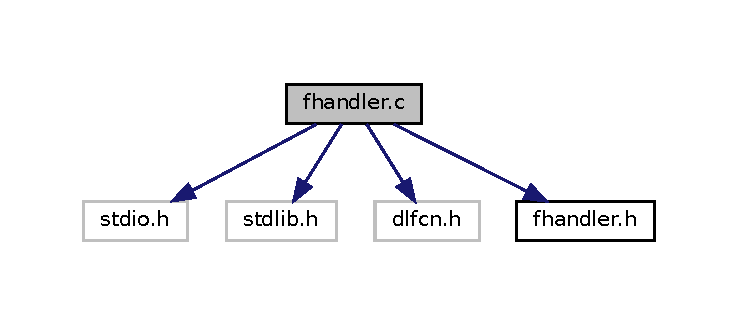
\includegraphics[width=350pt]{fhandler_8c__incl}
\end{center}
\end{figure}
\subsection*{Functions}
\begin{DoxyCompactItemize}
\item 
void \hyperlink{fhandler_8c_a9b1ada6e94cd79a619e282d13b8529d7_a9b1ada6e94cd79a619e282d13b8529d7}{Handle} (const char $\ast$\+\_\+\+\_\+lib, const char $\ast$\+\_\+\+\_\+func, void $\ast$\+\_\+funcp)
\begin{DoxyCompactList}\small\item\em Handles the dynamic linking of the functions. \end{DoxyCompactList}\end{DoxyCompactItemize}


\subsection{Function Documentation}
\mbox{\Hypertarget{fhandler_8c_a9b1ada6e94cd79a619e282d13b8529d7_a9b1ada6e94cd79a619e282d13b8529d7}\label{fhandler_8c_a9b1ada6e94cd79a619e282d13b8529d7_a9b1ada6e94cd79a619e282d13b8529d7}} 
\index{fhandler.\+c@{fhandler.\+c}!Handle@{Handle}}
\index{Handle@{Handle}!fhandler.\+c@{fhandler.\+c}}
\subsubsection{\texorpdfstring{Handle()}{Handle()}}
{\footnotesize\ttfamily void Handle (\begin{DoxyParamCaption}\item[{const char $\ast$}]{\+\_\+\+\_\+lib,  }\item[{const char $\ast$}]{\+\_\+\+\_\+func,  }\item[{void $\ast$}]{\+\_\+funcp }\end{DoxyParamCaption})}



Handles the dynamic linking of the functions. 


\begin{DoxyParams}{Parameters}
{\em \+\_\+\+\_\+lib} & The library name to be linked. \\
\hline
{\em \+\_\+\+\_\+func} & The function name to be linked. \\
\hline
{\em \+\_\+funcp} & The pointer to the function to be linked. \\
\hline
\end{DoxyParams}

\hypertarget{fhandler_8h}{}\section{fhandler.\+h File Reference}
\label{fhandler_8h}\index{fhandler.\+h@{fhandler.\+h}}
This graph shows which files directly or indirectly include this file\+:\nopagebreak
\begin{figure}[H]
\begin{center}
\leavevmode
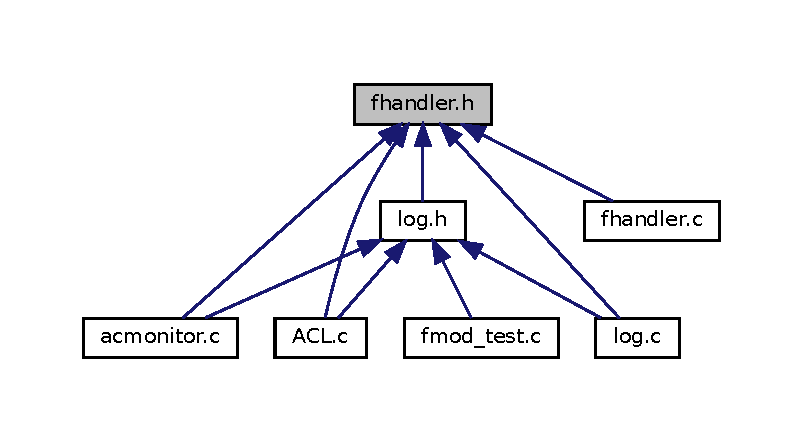
\includegraphics[width=350pt]{fhandler_8h__dep__incl}
\end{center}
\end{figure}
\subsection*{Macros}
\begin{DoxyCompactItemize}
\item 
\#define \hyperlink{fhandler_8h_a369266c24eacffb87046522897a570d5_a369266c24eacffb87046522897a570d5}{\+\_\+\+G\+N\+U\+\_\+\+S\+O\+U\+R\+CE}
\end{DoxyCompactItemize}
\subsection*{Functions}
\begin{DoxyCompactItemize}
\item 
void \hyperlink{fhandler_8h_a9b1ada6e94cd79a619e282d13b8529d7_a9b1ada6e94cd79a619e282d13b8529d7}{Handle} (const char $\ast$\+\_\+\+\_\+lib, const char $\ast$\+\_\+\+\_\+func, void $\ast$\+\_\+funcp)
\begin{DoxyCompactList}\small\item\em Handles the dynamic linking of the functions. \end{DoxyCompactList}\end{DoxyCompactItemize}


\subsection{Macro Definition Documentation}
\mbox{\Hypertarget{fhandler_8h_a369266c24eacffb87046522897a570d5_a369266c24eacffb87046522897a570d5}\label{fhandler_8h_a369266c24eacffb87046522897a570d5_a369266c24eacffb87046522897a570d5}} 
\index{fhandler.\+h@{fhandler.\+h}!\+\_\+\+G\+N\+U\+\_\+\+S\+O\+U\+R\+CE@{\+\_\+\+G\+N\+U\+\_\+\+S\+O\+U\+R\+CE}}
\index{\+\_\+\+G\+N\+U\+\_\+\+S\+O\+U\+R\+CE@{\+\_\+\+G\+N\+U\+\_\+\+S\+O\+U\+R\+CE}!fhandler.\+h@{fhandler.\+h}}
\subsubsection{\texorpdfstring{\+\_\+\+G\+N\+U\+\_\+\+S\+O\+U\+R\+CE}{\_GNU\_SOURCE}}
{\footnotesize\ttfamily \#define \+\_\+\+G\+N\+U\+\_\+\+S\+O\+U\+R\+CE}



\subsection{Function Documentation}
\mbox{\Hypertarget{fhandler_8h_a9b1ada6e94cd79a619e282d13b8529d7_a9b1ada6e94cd79a619e282d13b8529d7}\label{fhandler_8h_a9b1ada6e94cd79a619e282d13b8529d7_a9b1ada6e94cd79a619e282d13b8529d7}} 
\index{fhandler.\+h@{fhandler.\+h}!Handle@{Handle}}
\index{Handle@{Handle}!fhandler.\+h@{fhandler.\+h}}
\subsubsection{\texorpdfstring{Handle()}{Handle()}}
{\footnotesize\ttfamily void Handle (\begin{DoxyParamCaption}\item[{const char $\ast$}]{\+\_\+\+\_\+lib,  }\item[{const char $\ast$}]{\+\_\+\+\_\+func,  }\item[{void $\ast$}]{\+\_\+funcp }\end{DoxyParamCaption})}



Handles the dynamic linking of the functions. 


\begin{DoxyParams}{Parameters}
{\em \+\_\+\+\_\+lib} & The library name to be linked. \\
\hline
{\em \+\_\+\+\_\+func} & The function name to be linked. \\
\hline
{\em \+\_\+funcp} & The pointer to the function to be linked. \\
\hline
\end{DoxyParams}

\hypertarget{fmod__test_8c}{}\section{fmod\+\_\+test.\+c File Reference}
\label{fmod__test_8c}\index{fmod\+\_\+test.\+c@{fmod\+\_\+test.\+c}}
{\ttfamily \#include $<$sys/types.\+h$>$}\newline
{\ttfamily \#include $<$sys/stat.\+h$>$}\newline
{\ttfamily \#include $<$unistd.\+h$>$}\newline
{\ttfamily \#include $<$stdio.\+h$>$}\newline
{\ttfamily \#include \char`\"{}../lib/\+Misc.\+h\char`\"{}}\newline
{\ttfamily \#include \char`\"{}../lib/log.\+h\char`\"{}}\newline
{\ttfamily \#include $<$stdlib.\+h$>$}\newline
{\ttfamily \#include $<$string.\+h$>$}\newline
Include dependency graph for fmod\+\_\+test.\+c\+:\nopagebreak
\begin{figure}[H]
\begin{center}
\leavevmode
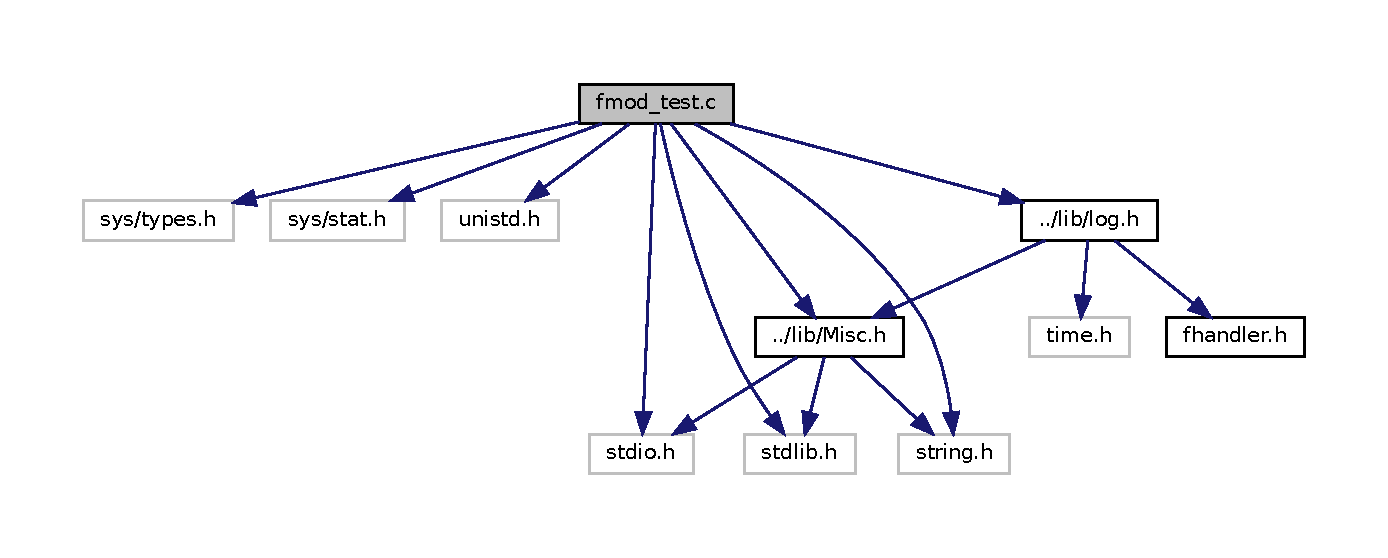
\includegraphics[width=350pt]{fmod__test_8c__incl}
\end{center}
\end{figure}
\subsection*{Macros}
\begin{DoxyCompactItemize}
\item 
\#define \hyperlink{fmod__test_8c_ac4c027058e9ccd1d4dce6a718af0b422_ac4c027058e9ccd1d4dce6a718af0b422}{printd}(format, ...)
\item 
\#define \hyperlink{fmod__test_8c_a8b3a3c4c8735fffe0d3b0ab6c7053667_a8b3a3c4c8735fffe0d3b0ab6c7053667}{printld}(format, ...)
\item 
\#define \hyperlink{fmod__test_8c_a483d4c865c4cb956ffe919f48867641a_a483d4c865c4cb956ffe919f48867641a}{printv}(format, ...)
\item 
\#define \hyperlink{fmod__test_8c_a8d23feea868a983c8c2b661e1e16972f_a8d23feea868a983c8c2b661e1e16972f}{R\+ED}~\char`\"{}\textbackslash{}x1B\mbox{[}31m\char`\"{}
\item 
\#define \hyperlink{fmod__test_8c_aea69ffbacdcdf16c21b8c9961df84448_aea69ffbacdcdf16c21b8c9961df84448}{G\+RN}~\char`\"{}\textbackslash{}x1B\mbox{[}32m\char`\"{}
\item 
\#define \hyperlink{fmod__test_8c_a96fac03c4ab3363f06a0328e0e53a40c_a96fac03c4ab3363f06a0328e0e53a40c}{Y\+EL}~\char`\"{}\textbackslash{}x1B\mbox{[}33m\char`\"{}
\item 
\#define \hyperlink{fmod__test_8c_add9307de87f38e77d336751e305886f6_add9307de87f38e77d336751e305886f6}{B\+LU}~\char`\"{}\textbackslash{}x1B\mbox{[}34m\char`\"{}
\item 
\#define \hyperlink{fmod__test_8c_af54a5a977c0c499323d656315f008ee0_af54a5a977c0c499323d656315f008ee0}{M\+AG}~\char`\"{}\textbackslash{}x1B\mbox{[}35m\char`\"{}
\item 
\#define \hyperlink{fmod__test_8c_adc708fa688f5d78db361f66c36f0f807_adc708fa688f5d78db361f66c36f0f807}{C\+YN}~\char`\"{}\textbackslash{}x1B\mbox{[}36m\char`\"{}
\item 
\#define \hyperlink{fmod__test_8c_aeaf3a04d5bf63b204689a714718ea930_aeaf3a04d5bf63b204689a714718ea930}{W\+HT}~\char`\"{}\textbackslash{}x1B\mbox{[}37m\char`\"{}
\item 
\#define \hyperlink{fmod__test_8c_ab702106cf3b3e96750b6845ded4e0299_ab702106cf3b3e96750b6845ded4e0299}{R\+E\+S\+ET}~\char`\"{}\textbackslash{}x1B\mbox{[}0m\char`\"{}
\end{DoxyCompactItemize}
\subsection*{Functions}
\begin{DoxyCompactItemize}
\item 
int \hyperlink{fmod__test_8c_aca3a9fb5c41af904fa57742f8a9e9b15_aca3a9fb5c41af904fa57742f8a9e9b15}{Write} ()
\item 
int \hyperlink{fmod__test_8c_a840291bc02cba5474a4cb46a9b9566fe_a840291bc02cba5474a4cb46a9b9566fe}{main} (void)
\end{DoxyCompactItemize}
\subsection*{Variables}
\begin{DoxyCompactItemize}
\item 
char $\ast$ \hyperlink{fmod__test_8c_a63b532db3eeff7bcfc7ac922342e7e22_a63b532db3eeff7bcfc7ac922342e7e22}{chat\+G\+P\+T\+\_\+is\+\_\+a\+\_\+poet} \mbox{[}$\,$\mbox{]}
\end{DoxyCompactItemize}


\subsection{Macro Definition Documentation}
\mbox{\Hypertarget{fmod__test_8c_add9307de87f38e77d336751e305886f6_add9307de87f38e77d336751e305886f6}\label{fmod__test_8c_add9307de87f38e77d336751e305886f6_add9307de87f38e77d336751e305886f6}} 
\index{fmod\+\_\+test.\+c@{fmod\+\_\+test.\+c}!B\+LU@{B\+LU}}
\index{B\+LU@{B\+LU}!fmod\+\_\+test.\+c@{fmod\+\_\+test.\+c}}
\subsubsection{\texorpdfstring{B\+LU}{BLU}}
{\footnotesize\ttfamily \#define B\+LU~\char`\"{}\textbackslash{}x1B\mbox{[}34m\char`\"{}}

\mbox{\Hypertarget{fmod__test_8c_adc708fa688f5d78db361f66c36f0f807_adc708fa688f5d78db361f66c36f0f807}\label{fmod__test_8c_adc708fa688f5d78db361f66c36f0f807_adc708fa688f5d78db361f66c36f0f807}} 
\index{fmod\+\_\+test.\+c@{fmod\+\_\+test.\+c}!C\+YN@{C\+YN}}
\index{C\+YN@{C\+YN}!fmod\+\_\+test.\+c@{fmod\+\_\+test.\+c}}
\subsubsection{\texorpdfstring{C\+YN}{CYN}}
{\footnotesize\ttfamily \#define C\+YN~\char`\"{}\textbackslash{}x1B\mbox{[}36m\char`\"{}}

\mbox{\Hypertarget{fmod__test_8c_aea69ffbacdcdf16c21b8c9961df84448_aea69ffbacdcdf16c21b8c9961df84448}\label{fmod__test_8c_aea69ffbacdcdf16c21b8c9961df84448_aea69ffbacdcdf16c21b8c9961df84448}} 
\index{fmod\+\_\+test.\+c@{fmod\+\_\+test.\+c}!G\+RN@{G\+RN}}
\index{G\+RN@{G\+RN}!fmod\+\_\+test.\+c@{fmod\+\_\+test.\+c}}
\subsubsection{\texorpdfstring{G\+RN}{GRN}}
{\footnotesize\ttfamily \#define G\+RN~\char`\"{}\textbackslash{}x1B\mbox{[}32m\char`\"{}}

\mbox{\Hypertarget{fmod__test_8c_af54a5a977c0c499323d656315f008ee0_af54a5a977c0c499323d656315f008ee0}\label{fmod__test_8c_af54a5a977c0c499323d656315f008ee0_af54a5a977c0c499323d656315f008ee0}} 
\index{fmod\+\_\+test.\+c@{fmod\+\_\+test.\+c}!M\+AG@{M\+AG}}
\index{M\+AG@{M\+AG}!fmod\+\_\+test.\+c@{fmod\+\_\+test.\+c}}
\subsubsection{\texorpdfstring{M\+AG}{MAG}}
{\footnotesize\ttfamily \#define M\+AG~\char`\"{}\textbackslash{}x1B\mbox{[}35m\char`\"{}}

\mbox{\Hypertarget{fmod__test_8c_ac4c027058e9ccd1d4dce6a718af0b422_ac4c027058e9ccd1d4dce6a718af0b422}\label{fmod__test_8c_ac4c027058e9ccd1d4dce6a718af0b422_ac4c027058e9ccd1d4dce6a718af0b422}} 
\index{fmod\+\_\+test.\+c@{fmod\+\_\+test.\+c}!printd@{printd}}
\index{printd@{printd}!fmod\+\_\+test.\+c@{fmod\+\_\+test.\+c}}
\subsubsection{\texorpdfstring{printd}{printd}}
{\footnotesize\ttfamily \#define printd(\begin{DoxyParamCaption}\item[{}]{format,  }\item[{}]{... }\end{DoxyParamCaption})}

\mbox{\Hypertarget{fmod__test_8c_a8b3a3c4c8735fffe0d3b0ab6c7053667_a8b3a3c4c8735fffe0d3b0ab6c7053667}\label{fmod__test_8c_a8b3a3c4c8735fffe0d3b0ab6c7053667_a8b3a3c4c8735fffe0d3b0ab6c7053667}} 
\index{fmod\+\_\+test.\+c@{fmod\+\_\+test.\+c}!printld@{printld}}
\index{printld@{printld}!fmod\+\_\+test.\+c@{fmod\+\_\+test.\+c}}
\subsubsection{\texorpdfstring{printld}{printld}}
{\footnotesize\ttfamily \#define printld(\begin{DoxyParamCaption}\item[{}]{format,  }\item[{}]{... }\end{DoxyParamCaption})}

\mbox{\Hypertarget{fmod__test_8c_a483d4c865c4cb956ffe919f48867641a_a483d4c865c4cb956ffe919f48867641a}\label{fmod__test_8c_a483d4c865c4cb956ffe919f48867641a_a483d4c865c4cb956ffe919f48867641a}} 
\index{fmod\+\_\+test.\+c@{fmod\+\_\+test.\+c}!printv@{printv}}
\index{printv@{printv}!fmod\+\_\+test.\+c@{fmod\+\_\+test.\+c}}
\subsubsection{\texorpdfstring{printv}{printv}}
{\footnotesize\ttfamily \#define printv(\begin{DoxyParamCaption}\item[{}]{format,  }\item[{}]{... }\end{DoxyParamCaption})}

\mbox{\Hypertarget{fmod__test_8c_a8d23feea868a983c8c2b661e1e16972f_a8d23feea868a983c8c2b661e1e16972f}\label{fmod__test_8c_a8d23feea868a983c8c2b661e1e16972f_a8d23feea868a983c8c2b661e1e16972f}} 
\index{fmod\+\_\+test.\+c@{fmod\+\_\+test.\+c}!R\+ED@{R\+ED}}
\index{R\+ED@{R\+ED}!fmod\+\_\+test.\+c@{fmod\+\_\+test.\+c}}
\subsubsection{\texorpdfstring{R\+ED}{RED}}
{\footnotesize\ttfamily \#define R\+ED~\char`\"{}\textbackslash{}x1B\mbox{[}31m\char`\"{}}

\mbox{\Hypertarget{fmod__test_8c_ab702106cf3b3e96750b6845ded4e0299_ab702106cf3b3e96750b6845ded4e0299}\label{fmod__test_8c_ab702106cf3b3e96750b6845ded4e0299_ab702106cf3b3e96750b6845ded4e0299}} 
\index{fmod\+\_\+test.\+c@{fmod\+\_\+test.\+c}!R\+E\+S\+ET@{R\+E\+S\+ET}}
\index{R\+E\+S\+ET@{R\+E\+S\+ET}!fmod\+\_\+test.\+c@{fmod\+\_\+test.\+c}}
\subsubsection{\texorpdfstring{R\+E\+S\+ET}{RESET}}
{\footnotesize\ttfamily \#define R\+E\+S\+ET~\char`\"{}\textbackslash{}x1B\mbox{[}0m\char`\"{}}

\mbox{\Hypertarget{fmod__test_8c_aeaf3a04d5bf63b204689a714718ea930_aeaf3a04d5bf63b204689a714718ea930}\label{fmod__test_8c_aeaf3a04d5bf63b204689a714718ea930_aeaf3a04d5bf63b204689a714718ea930}} 
\index{fmod\+\_\+test.\+c@{fmod\+\_\+test.\+c}!W\+HT@{W\+HT}}
\index{W\+HT@{W\+HT}!fmod\+\_\+test.\+c@{fmod\+\_\+test.\+c}}
\subsubsection{\texorpdfstring{W\+HT}{WHT}}
{\footnotesize\ttfamily \#define W\+HT~\char`\"{}\textbackslash{}x1B\mbox{[}37m\char`\"{}}

\mbox{\Hypertarget{fmod__test_8c_a96fac03c4ab3363f06a0328e0e53a40c_a96fac03c4ab3363f06a0328e0e53a40c}\label{fmod__test_8c_a96fac03c4ab3363f06a0328e0e53a40c_a96fac03c4ab3363f06a0328e0e53a40c}} 
\index{fmod\+\_\+test.\+c@{fmod\+\_\+test.\+c}!Y\+EL@{Y\+EL}}
\index{Y\+EL@{Y\+EL}!fmod\+\_\+test.\+c@{fmod\+\_\+test.\+c}}
\subsubsection{\texorpdfstring{Y\+EL}{YEL}}
{\footnotesize\ttfamily \#define Y\+EL~\char`\"{}\textbackslash{}x1B\mbox{[}33m\char`\"{}}



\subsection{Function Documentation}
\mbox{\Hypertarget{fmod__test_8c_a840291bc02cba5474a4cb46a9b9566fe_a840291bc02cba5474a4cb46a9b9566fe}\label{fmod__test_8c_a840291bc02cba5474a4cb46a9b9566fe_a840291bc02cba5474a4cb46a9b9566fe}} 
\index{fmod\+\_\+test.\+c@{fmod\+\_\+test.\+c}!main@{main}}
\index{main@{main}!fmod\+\_\+test.\+c@{fmod\+\_\+test.\+c}}
\subsubsection{\texorpdfstring{main()}{main()}}
{\footnotesize\ttfamily int main (\begin{DoxyParamCaption}\item[{void}]{ }\end{DoxyParamCaption})}

\mbox{\Hypertarget{fmod__test_8c_aca3a9fb5c41af904fa57742f8a9e9b15_aca3a9fb5c41af904fa57742f8a9e9b15}\label{fmod__test_8c_aca3a9fb5c41af904fa57742f8a9e9b15_aca3a9fb5c41af904fa57742f8a9e9b15}} 
\index{fmod\+\_\+test.\+c@{fmod\+\_\+test.\+c}!Write@{Write}}
\index{Write@{Write}!fmod\+\_\+test.\+c@{fmod\+\_\+test.\+c}}
\subsubsection{\texorpdfstring{Write()}{Write()}}
{\footnotesize\ttfamily int Write (\begin{DoxyParamCaption}{ }\end{DoxyParamCaption})}



\subsection{Variable Documentation}
\mbox{\Hypertarget{fmod__test_8c_a63b532db3eeff7bcfc7ac922342e7e22_a63b532db3eeff7bcfc7ac922342e7e22}\label{fmod__test_8c_a63b532db3eeff7bcfc7ac922342e7e22_a63b532db3eeff7bcfc7ac922342e7e22}} 
\index{fmod\+\_\+test.\+c@{fmod\+\_\+test.\+c}!chat\+G\+P\+T\+\_\+is\+\_\+a\+\_\+poet@{chat\+G\+P\+T\+\_\+is\+\_\+a\+\_\+poet}}
\index{chat\+G\+P\+T\+\_\+is\+\_\+a\+\_\+poet@{chat\+G\+P\+T\+\_\+is\+\_\+a\+\_\+poet}!fmod\+\_\+test.\+c@{fmod\+\_\+test.\+c}}
\subsubsection{\texorpdfstring{chat\+G\+P\+T\+\_\+is\+\_\+a\+\_\+poet}{chatGPT\_is\_a\_poet}}
{\footnotesize\ttfamily char$\ast$ chat\+G\+P\+T\+\_\+is\+\_\+a\+\_\+poet\mbox{[}$\,$\mbox{]}}

In this test we are going to test the modification monitor \hyperlink{acmonitor_8c}{acmonitor.\+c} !!! .

We are going to write 41 lines of text to a file line by line. Each time we mark the number of accesses to the file before and after we write the lines, and at the end we see whether the number of accesses is correct. 
\hypertarget{fperm__test_8c}{}\section{fperm\+\_\+test.\+c File Reference}
\label{fperm__test_8c}\index{fperm\+\_\+test.\+c@{fperm\+\_\+test.\+c}}
{\ttfamily \#include $<$sys/types.\+h$>$}\newline
{\ttfamily \#include $<$sys/stat.\+h$>$}\newline
{\ttfamily \#include $<$unistd.\+h$>$}\newline
{\ttfamily \#include $<$stdio.\+h$>$}\newline
{\ttfamily \#include $<$grp.\+h$>$}\newline
{\ttfamily \#include $<$pwd.\+h$>$}\newline
{\ttfamily \#include $<$errno.\+h$>$}\newline
{\ttfamily \#include $<$stdlib.\+h$>$}\newline
{\ttfamily \#include $<$string.\+h$>$}\newline
Include dependency graph for fperm\+\_\+test.\+c\+:\nopagebreak
\begin{figure}[H]
\begin{center}
\leavevmode
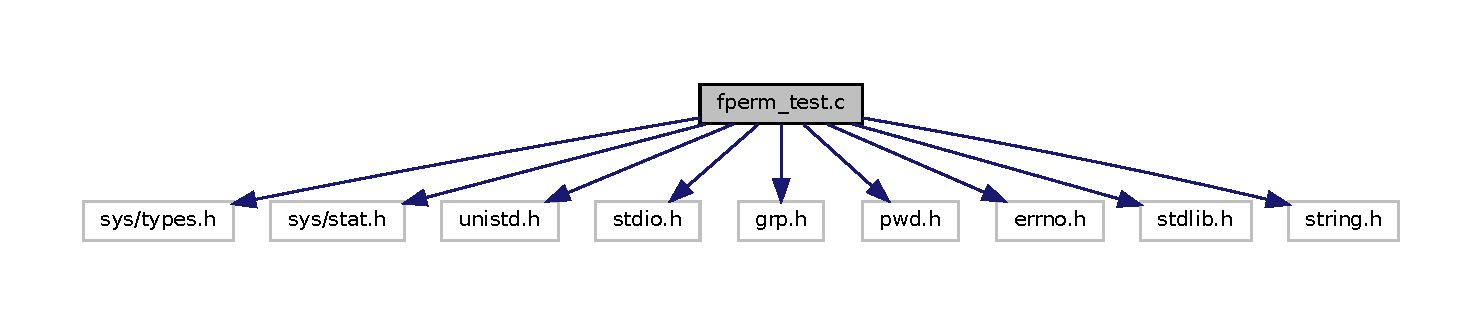
\includegraphics[width=350pt]{fperm__test_8c__incl}
\end{center}
\end{figure}
\subsection*{Macros}
\begin{DoxyCompactItemize}
\item 
\#define \hyperlink{fperm__test_8c_a8d23feea868a983c8c2b661e1e16972f_a8d23feea868a983c8c2b661e1e16972f}{R\+ED}~\char`\"{}\textbackslash{}x1B\mbox{[}31m\char`\"{}
\item 
\#define \hyperlink{fperm__test_8c_aea69ffbacdcdf16c21b8c9961df84448_aea69ffbacdcdf16c21b8c9961df84448}{G\+RN}~\char`\"{}\textbackslash{}x1B\mbox{[}32m\char`\"{}
\item 
\#define \hyperlink{fperm__test_8c_a96fac03c4ab3363f06a0328e0e53a40c_a96fac03c4ab3363f06a0328e0e53a40c}{Y\+EL}~\char`\"{}\textbackslash{}x1B\mbox{[}33m\char`\"{}
\item 
\#define \hyperlink{fperm__test_8c_add9307de87f38e77d336751e305886f6_add9307de87f38e77d336751e305886f6}{B\+LU}~\char`\"{}\textbackslash{}x1B\mbox{[}34m\char`\"{}
\item 
\#define \hyperlink{fperm__test_8c_af54a5a977c0c499323d656315f008ee0_af54a5a977c0c499323d656315f008ee0}{M\+AG}~\char`\"{}\textbackslash{}x1B\mbox{[}35m\char`\"{}
\item 
\#define \hyperlink{fperm__test_8c_adc708fa688f5d78db361f66c36f0f807_adc708fa688f5d78db361f66c36f0f807}{C\+YN}~\char`\"{}\textbackslash{}x1B\mbox{[}36m\char`\"{}
\item 
\#define \hyperlink{fperm__test_8c_aeaf3a04d5bf63b204689a714718ea930_aeaf3a04d5bf63b204689a714718ea930}{W\+HT}~\char`\"{}\textbackslash{}x1B\mbox{[}37m\char`\"{}
\item 
\#define \hyperlink{fperm__test_8c_ab702106cf3b3e96750b6845ded4e0299_ab702106cf3b3e96750b6845ded4e0299}{R\+E\+S\+ET}~\char`\"{}\textbackslash{}x1B\mbox{[}0m\char`\"{}
\end{DoxyCompactItemize}
\subsection*{Functions}
\begin{DoxyCompactItemize}
\item 
int \hyperlink{fperm__test_8c_a711d0bb2170aecd6cda15f498aa8660f_a711d0bb2170aecd6cda15f498aa8660f}{test\+Write} ()
\item 
int \hyperlink{fperm__test_8c_a82c9fc590374ae3e8a847687266c8537_a82c9fc590374ae3e8a847687266c8537}{test\+Read} ()
\item 
int \hyperlink{fperm__test_8c_a4c730ced6041a87cf27be08a5cc591af_a4c730ced6041a87cf27be08a5cc591af}{test\+Exec} ()
\item 
int \hyperlink{fperm__test_8c_ae66f6b31b5ad750f1fe042a706a4e3d4_ae66f6b31b5ad750f1fe042a706a4e3d4}{main} ()
\end{DoxyCompactItemize}
\subsection*{Variables}
\begin{DoxyCompactItemize}
\item 
char \hyperlink{fperm__test_8c_a9acefa3eb5b801834cb9b7a7453b41e0_a9acefa3eb5b801834cb9b7a7453b41e0}{paths} \mbox{[}$\,$\mbox{]}\mbox{[}256\mbox{]}
\end{DoxyCompactItemize}


\subsection{Macro Definition Documentation}
\mbox{\Hypertarget{fperm__test_8c_add9307de87f38e77d336751e305886f6_add9307de87f38e77d336751e305886f6}\label{fperm__test_8c_add9307de87f38e77d336751e305886f6_add9307de87f38e77d336751e305886f6}} 
\index{fperm\+\_\+test.\+c@{fperm\+\_\+test.\+c}!B\+LU@{B\+LU}}
\index{B\+LU@{B\+LU}!fperm\+\_\+test.\+c@{fperm\+\_\+test.\+c}}
\subsubsection{\texorpdfstring{B\+LU}{BLU}}
{\footnotesize\ttfamily \#define B\+LU~\char`\"{}\textbackslash{}x1B\mbox{[}34m\char`\"{}}

\mbox{\Hypertarget{fperm__test_8c_adc708fa688f5d78db361f66c36f0f807_adc708fa688f5d78db361f66c36f0f807}\label{fperm__test_8c_adc708fa688f5d78db361f66c36f0f807_adc708fa688f5d78db361f66c36f0f807}} 
\index{fperm\+\_\+test.\+c@{fperm\+\_\+test.\+c}!C\+YN@{C\+YN}}
\index{C\+YN@{C\+YN}!fperm\+\_\+test.\+c@{fperm\+\_\+test.\+c}}
\subsubsection{\texorpdfstring{C\+YN}{CYN}}
{\footnotesize\ttfamily \#define C\+YN~\char`\"{}\textbackslash{}x1B\mbox{[}36m\char`\"{}}

\mbox{\Hypertarget{fperm__test_8c_aea69ffbacdcdf16c21b8c9961df84448_aea69ffbacdcdf16c21b8c9961df84448}\label{fperm__test_8c_aea69ffbacdcdf16c21b8c9961df84448_aea69ffbacdcdf16c21b8c9961df84448}} 
\index{fperm\+\_\+test.\+c@{fperm\+\_\+test.\+c}!G\+RN@{G\+RN}}
\index{G\+RN@{G\+RN}!fperm\+\_\+test.\+c@{fperm\+\_\+test.\+c}}
\subsubsection{\texorpdfstring{G\+RN}{GRN}}
{\footnotesize\ttfamily \#define G\+RN~\char`\"{}\textbackslash{}x1B\mbox{[}32m\char`\"{}}

\mbox{\Hypertarget{fperm__test_8c_af54a5a977c0c499323d656315f008ee0_af54a5a977c0c499323d656315f008ee0}\label{fperm__test_8c_af54a5a977c0c499323d656315f008ee0_af54a5a977c0c499323d656315f008ee0}} 
\index{fperm\+\_\+test.\+c@{fperm\+\_\+test.\+c}!M\+AG@{M\+AG}}
\index{M\+AG@{M\+AG}!fperm\+\_\+test.\+c@{fperm\+\_\+test.\+c}}
\subsubsection{\texorpdfstring{M\+AG}{MAG}}
{\footnotesize\ttfamily \#define M\+AG~\char`\"{}\textbackslash{}x1B\mbox{[}35m\char`\"{}}

\mbox{\Hypertarget{fperm__test_8c_a8d23feea868a983c8c2b661e1e16972f_a8d23feea868a983c8c2b661e1e16972f}\label{fperm__test_8c_a8d23feea868a983c8c2b661e1e16972f_a8d23feea868a983c8c2b661e1e16972f}} 
\index{fperm\+\_\+test.\+c@{fperm\+\_\+test.\+c}!R\+ED@{R\+ED}}
\index{R\+ED@{R\+ED}!fperm\+\_\+test.\+c@{fperm\+\_\+test.\+c}}
\subsubsection{\texorpdfstring{R\+ED}{RED}}
{\footnotesize\ttfamily \#define R\+ED~\char`\"{}\textbackslash{}x1B\mbox{[}31m\char`\"{}}

\mbox{\Hypertarget{fperm__test_8c_ab702106cf3b3e96750b6845ded4e0299_ab702106cf3b3e96750b6845ded4e0299}\label{fperm__test_8c_ab702106cf3b3e96750b6845ded4e0299_ab702106cf3b3e96750b6845ded4e0299}} 
\index{fperm\+\_\+test.\+c@{fperm\+\_\+test.\+c}!R\+E\+S\+ET@{R\+E\+S\+ET}}
\index{R\+E\+S\+ET@{R\+E\+S\+ET}!fperm\+\_\+test.\+c@{fperm\+\_\+test.\+c}}
\subsubsection{\texorpdfstring{R\+E\+S\+ET}{RESET}}
{\footnotesize\ttfamily \#define R\+E\+S\+ET~\char`\"{}\textbackslash{}x1B\mbox{[}0m\char`\"{}}

\mbox{\Hypertarget{fperm__test_8c_aeaf3a04d5bf63b204689a714718ea930_aeaf3a04d5bf63b204689a714718ea930}\label{fperm__test_8c_aeaf3a04d5bf63b204689a714718ea930_aeaf3a04d5bf63b204689a714718ea930}} 
\index{fperm\+\_\+test.\+c@{fperm\+\_\+test.\+c}!W\+HT@{W\+HT}}
\index{W\+HT@{W\+HT}!fperm\+\_\+test.\+c@{fperm\+\_\+test.\+c}}
\subsubsection{\texorpdfstring{W\+HT}{WHT}}
{\footnotesize\ttfamily \#define W\+HT~\char`\"{}\textbackslash{}x1B\mbox{[}37m\char`\"{}}

\mbox{\Hypertarget{fperm__test_8c_a96fac03c4ab3363f06a0328e0e53a40c_a96fac03c4ab3363f06a0328e0e53a40c}\label{fperm__test_8c_a96fac03c4ab3363f06a0328e0e53a40c_a96fac03c4ab3363f06a0328e0e53a40c}} 
\index{fperm\+\_\+test.\+c@{fperm\+\_\+test.\+c}!Y\+EL@{Y\+EL}}
\index{Y\+EL@{Y\+EL}!fperm\+\_\+test.\+c@{fperm\+\_\+test.\+c}}
\subsubsection{\texorpdfstring{Y\+EL}{YEL}}
{\footnotesize\ttfamily \#define Y\+EL~\char`\"{}\textbackslash{}x1B\mbox{[}33m\char`\"{}}



\subsection{Function Documentation}
\mbox{\Hypertarget{fperm__test_8c_ae66f6b31b5ad750f1fe042a706a4e3d4_ae66f6b31b5ad750f1fe042a706a4e3d4}\label{fperm__test_8c_ae66f6b31b5ad750f1fe042a706a4e3d4_ae66f6b31b5ad750f1fe042a706a4e3d4}} 
\index{fperm\+\_\+test.\+c@{fperm\+\_\+test.\+c}!main@{main}}
\index{main@{main}!fperm\+\_\+test.\+c@{fperm\+\_\+test.\+c}}
\subsubsection{\texorpdfstring{main()}{main()}}
{\footnotesize\ttfamily int main (\begin{DoxyParamCaption}\item[{void}]{ }\end{DoxyParamCaption})}

\mbox{\Hypertarget{fperm__test_8c_a4c730ced6041a87cf27be08a5cc591af_a4c730ced6041a87cf27be08a5cc591af}\label{fperm__test_8c_a4c730ced6041a87cf27be08a5cc591af_a4c730ced6041a87cf27be08a5cc591af}} 
\index{fperm\+\_\+test.\+c@{fperm\+\_\+test.\+c}!test\+Exec@{test\+Exec}}
\index{test\+Exec@{test\+Exec}!fperm\+\_\+test.\+c@{fperm\+\_\+test.\+c}}
\subsubsection{\texorpdfstring{test\+Exec()}{testExec()}}
{\footnotesize\ttfamily int test\+Exec (\begin{DoxyParamCaption}{ }\end{DoxyParamCaption})}

\mbox{\Hypertarget{fperm__test_8c_a82c9fc590374ae3e8a847687266c8537_a82c9fc590374ae3e8a847687266c8537}\label{fperm__test_8c_a82c9fc590374ae3e8a847687266c8537_a82c9fc590374ae3e8a847687266c8537}} 
\index{fperm\+\_\+test.\+c@{fperm\+\_\+test.\+c}!test\+Read@{test\+Read}}
\index{test\+Read@{test\+Read}!fperm\+\_\+test.\+c@{fperm\+\_\+test.\+c}}
\subsubsection{\texorpdfstring{test\+Read()}{testRead()}}
{\footnotesize\ttfamily int test\+Read (\begin{DoxyParamCaption}{ }\end{DoxyParamCaption})}

\mbox{\Hypertarget{fperm__test_8c_a711d0bb2170aecd6cda15f498aa8660f_a711d0bb2170aecd6cda15f498aa8660f}\label{fperm__test_8c_a711d0bb2170aecd6cda15f498aa8660f_a711d0bb2170aecd6cda15f498aa8660f}} 
\index{fperm\+\_\+test.\+c@{fperm\+\_\+test.\+c}!test\+Write@{test\+Write}}
\index{test\+Write@{test\+Write}!fperm\+\_\+test.\+c@{fperm\+\_\+test.\+c}}
\subsubsection{\texorpdfstring{test\+Write()}{testWrite()}}
{\footnotesize\ttfamily int test\+Write (\begin{DoxyParamCaption}{ }\end{DoxyParamCaption})}

In this test we check whether our program can bypass permissions.

We have created 18 files with different permissions and we try to read, write and execute them. 

\subsection{Variable Documentation}
\mbox{\Hypertarget{fperm__test_8c_a9acefa3eb5b801834cb9b7a7453b41e0_a9acefa3eb5b801834cb9b7a7453b41e0}\label{fperm__test_8c_a9acefa3eb5b801834cb9b7a7453b41e0_a9acefa3eb5b801834cb9b7a7453b41e0}} 
\index{fperm\+\_\+test.\+c@{fperm\+\_\+test.\+c}!paths@{paths}}
\index{paths@{paths}!fperm\+\_\+test.\+c@{fperm\+\_\+test.\+c}}
\subsubsection{\texorpdfstring{paths}{paths}}
{\footnotesize\ttfamily char paths\mbox{[}$\,$\mbox{]}\mbox{[}256\mbox{]}}

{\bfseries Initial value\+:}
\begin{DoxyCode}
= \{
    \textcolor{stringliteral}{"test/.testfiles/user\_read.c"},
    \textcolor{stringliteral}{"test/.testfiles/group\_read.c"},
    \textcolor{stringliteral}{"test/.testfiles/other\_read.c"},
    \textcolor{stringliteral}{"test/.testfiles/user\_write.c"},
    \textcolor{stringliteral}{"test/.testfiles/group\_write.c"},
    \textcolor{stringliteral}{"test/.testfiles/other\_write.c"},
    \textcolor{stringliteral}{"test/.testfiles/user\_execute"},
    \textcolor{stringliteral}{"test/.testfiles/group\_execute"},
    \textcolor{stringliteral}{"test/.testfiles/other\_execute"},
    \textcolor{stringliteral}{"test/.testfiles/user\_read\_write.c"},
    \textcolor{stringliteral}{"test/.testfiles/group\_read\_write.c"},
    \textcolor{stringliteral}{"test/.testfiles/other\_read\_write.c"},
    \textcolor{stringliteral}{"test/.testfiles/user\_read\_execute"},
    \textcolor{stringliteral}{"test/.testfiles/group\_read\_execute"},
    \textcolor{stringliteral}{"test/.testfiles/other\_read\_execute"},
    \textcolor{stringliteral}{"test/.testfiles/user\_write\_execute"},
    \textcolor{stringliteral}{"test/.testfiles/group\_write\_execute"},
    \textcolor{stringliteral}{"test/.testfiles/other\_write\_execute"}
\}
\end{DoxyCode}

\hypertarget{log_8c}{}\section{log.\+c File Reference}
\label{log_8c}\index{log.\+c@{log.\+c}}
{\ttfamily \#include \char`\"{}log.\+h\char`\"{}}\newline
{\ttfamily \#include $<$stdio.\+h$>$}\newline
{\ttfamily \#include $<$stdlib.\+h$>$}\newline
{\ttfamily \#include $<$string.\+h$>$}\newline
{\ttfamily \#include $<$dlfcn.\+h$>$}\newline
{\ttfamily \#include $<$time.\+h$>$}\newline
{\ttfamily \#include $<$unistd.\+h$>$}\newline
{\ttfamily \#include $<$stdarg.\+h$>$}\newline
{\ttfamily \#include \char`\"{}fhandler.\+h\char`\"{}}\newline
Include dependency graph for log.\+c\+:
\nopagebreak
\begin{figure}[H]
\begin{center}
\leavevmode
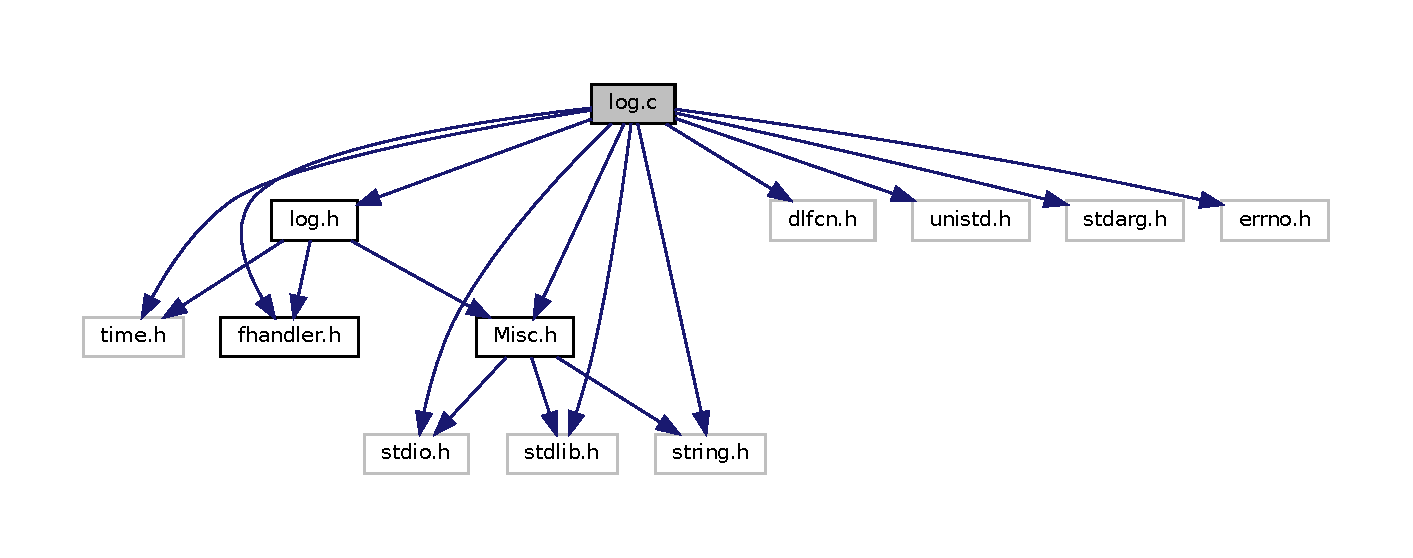
\includegraphics[width=350pt]{log_8c__incl}
\end{center}
\end{figure}
\subsection*{Functions}
\begin{DoxyCompactItemize}
\item 
struct tm \hyperlink{log_8c_a2de5fe84ca15039e1b007634ccef1651_a2de5fe84ca15039e1b007634ccef1651}{date\+\_\+and\+\_\+time} ()
\begin{DoxyCompactList}\small\item\em Create a timestamp object with the current date and time. \end{DoxyCompactList}\item 
void \hyperlink{log_8c_ab3a7d9a8e25e365afb72e557f60ba45f_ab3a7d9a8e25e365afb72e557f60ba45f}{print\+\_\+log\+\_\+to\+\_\+file} (\hyperlink{log_8h_abd600feddcc5ca71fa3f3afa84eee569_abd600feddcc5ca71fa3f3afa84eee569}{log\+\_\+t} \hyperlink{structlog__entry}{log\+\_\+entry})
\begin{DoxyCompactList}\small\item\em Prints the log entry to the log file. \end{DoxyCompactList}\item 
\hyperlink{log_8h_abd600feddcc5ca71fa3f3afa84eee569_abd600feddcc5ca71fa3f3afa84eee569}{log\+\_\+t} \hyperlink{log_8c_a208f5ebd87e3ff13ab84ab2d57c46974_a208f5ebd87e3ff13ab84ab2d57c46974}{create\+\_\+log} (const char $\ast$path, const \hyperlink{log_8h_ab20c54dfb1eb1323b9a3cfe2e6a76270_ab20c54dfb1eb1323b9a3cfe2e6a76270}{access\+\_\+t} access, const int action\+\_\+denied, unsigned char fingerprint\mbox{[}16\mbox{]})
\begin{DoxyCompactList}\small\item\em Creates a log entry. \end{DoxyCompactList}\end{DoxyCompactItemize}


\subsection{Function Documentation}
\mbox{\Hypertarget{log_8c_a208f5ebd87e3ff13ab84ab2d57c46974_a208f5ebd87e3ff13ab84ab2d57c46974}\label{log_8c_a208f5ebd87e3ff13ab84ab2d57c46974_a208f5ebd87e3ff13ab84ab2d57c46974}} 
\index{log.\+c@{log.\+c}!create\+\_\+log@{create\+\_\+log}}
\index{create\+\_\+log@{create\+\_\+log}!log.\+c@{log.\+c}}
\subsubsection{\texorpdfstring{create\+\_\+log()}{create\_log()}}
{\footnotesize\ttfamily \hyperlink{log_8h_abd600feddcc5ca71fa3f3afa84eee569_abd600feddcc5ca71fa3f3afa84eee569}{log\+\_\+t} create\+\_\+log (\begin{DoxyParamCaption}\item[{const char $\ast$}]{path,  }\item[{const \hyperlink{log_8h_ab20c54dfb1eb1323b9a3cfe2e6a76270_ab20c54dfb1eb1323b9a3cfe2e6a76270}{access\+\_\+t}}]{access,  }\item[{const int}]{action\+\_\+denied,  }\item[{unsigned char}]{fingerprint\mbox{[}16\mbox{]} }\end{DoxyParamCaption})}



Creates a log entry. 


\begin{DoxyParams}{Parameters}
{\em path} & The absolute path of the file. \\
\hline
{\em access} & The access type. see access\+\_\+t \\
\hline
{\em action\+\_\+denied} & 1 if the action was denied, else 0. \\
\hline
{\em fingerprint} & The fingerprint of the file. \\
\hline
\end{DoxyParams}
\mbox{\Hypertarget{log_8c_a2de5fe84ca15039e1b007634ccef1651_a2de5fe84ca15039e1b007634ccef1651}\label{log_8c_a2de5fe84ca15039e1b007634ccef1651_a2de5fe84ca15039e1b007634ccef1651}} 
\index{log.\+c@{log.\+c}!date\+\_\+and\+\_\+time@{date\+\_\+and\+\_\+time}}
\index{date\+\_\+and\+\_\+time@{date\+\_\+and\+\_\+time}!log.\+c@{log.\+c}}
\subsubsection{\texorpdfstring{date\+\_\+and\+\_\+time()}{date\_and\_time()}}
{\footnotesize\ttfamily struct tm date\+\_\+and\+\_\+time (\begin{DoxyParamCaption}{ }\end{DoxyParamCaption})}



Create a timestamp object with the current date and time. 

\begin{DoxyReturn}{Returns}
struct tm The current date and time. 
\end{DoxyReturn}
\mbox{\Hypertarget{log_8c_ab3a7d9a8e25e365afb72e557f60ba45f_ab3a7d9a8e25e365afb72e557f60ba45f}\label{log_8c_ab3a7d9a8e25e365afb72e557f60ba45f_ab3a7d9a8e25e365afb72e557f60ba45f}} 
\index{log.\+c@{log.\+c}!print\+\_\+log\+\_\+to\+\_\+file@{print\+\_\+log\+\_\+to\+\_\+file}}
\index{print\+\_\+log\+\_\+to\+\_\+file@{print\+\_\+log\+\_\+to\+\_\+file}!log.\+c@{log.\+c}}
\subsubsection{\texorpdfstring{print\+\_\+log\+\_\+to\+\_\+file()}{print\_log\_to\_file()}}
{\footnotesize\ttfamily void print\+\_\+log\+\_\+to\+\_\+file (\begin{DoxyParamCaption}\item[{\hyperlink{log_8h_abd600feddcc5ca71fa3f3afa84eee569_abd600feddcc5ca71fa3f3afa84eee569}{log\+\_\+t}}]{log\+\_\+entry }\end{DoxyParamCaption})}



Prints the log entry to the log file. 


\begin{DoxyParams}{Parameters}
{\em \hyperlink{structlog__entry}{log\+\_\+entry}} & The log entry to be printed. \\
\hline
\end{DoxyParams}

\hypertarget{log_8h}{}\section{log.\+h File Reference}
\label{log_8h}\index{log.\+h@{log.\+h}}
{\ttfamily \#include $<$time.\+h$>$}\newline
{\ttfamily \#include \char`\"{}fhandler.\+h\char`\"{}}\newline
{\ttfamily \#include \char`\"{}Misc.\+h\char`\"{}}\newline
Include dependency graph for log.\+h\+:\nopagebreak
\begin{figure}[H]
\begin{center}
\leavevmode
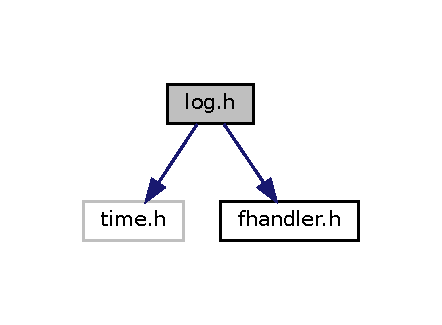
\includegraphics[width=350pt]{log_8h__incl}
\end{center}
\end{figure}
This graph shows which files directly or indirectly include this file\+:\nopagebreak
\begin{figure}[H]
\begin{center}
\leavevmode
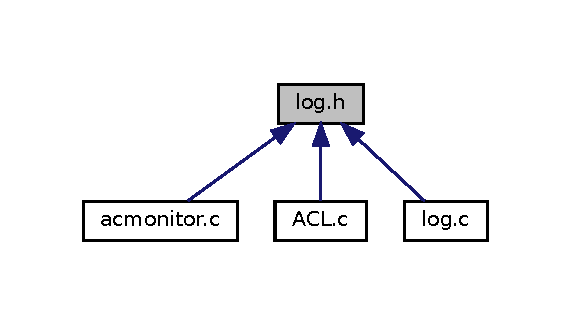
\includegraphics[width=350pt]{log_8h__dep__incl}
\end{center}
\end{figure}
\subsection*{Data Structures}
\begin{DoxyCompactItemize}
\item 
struct \hyperlink{structlog__entry}{log\+\_\+entry}
\begin{DoxyCompactList}\small\item\em The log entry. \end{DoxyCompactList}\item 
struct \hyperlink{structlog__entry__s}{log\+\_\+entry\+\_\+s}
\begin{DoxyCompactList}\small\item\em The log entry in strings format. \end{DoxyCompactList}\item 
struct \hyperlink{structuser__history}{user\+\_\+history}
\begin{DoxyCompactList}\small\item\em User history in the log. Contains all files the user attempted ro access or modify but was rejected. \end{DoxyCompactList}\item 
struct \hyperlink{structfile__history}{file\+\_\+history}
\begin{DoxyCompactList}\small\item\em File history in the log. Contains logs regarding a file. \end{DoxyCompactList}\end{DoxyCompactItemize}
\subsection*{Macros}
\begin{DoxyCompactItemize}
\item 
\#define \hyperlink{log_8h_a286c666b6725cb6f32fbd5500f41dd9f_a286c666b6725cb6f32fbd5500f41dd9f}{\+\_\+\+L\+O\+G\+\_\+\+F\+I\+L\+E\+\_\+\+P\+A\+T\+H\+\_\+}~\char`\"{}etc/log.\+txt\char`\"{}
\begin{DoxyCompactList}\small\item\em Handles all operations regarding the log file. \end{DoxyCompactList}\end{DoxyCompactItemize}
\subsection*{Typedefs}
\begin{DoxyCompactItemize}
\item 
typedef enum \hyperlink{log_8h_a1f5bf9b97a6a0e44df8bdfe6c9779e24_a1f5bf9b97a6a0e44df8bdfe6c9779e24}{access\+\_\+types} \hyperlink{log_8h_ab20c54dfb1eb1323b9a3cfe2e6a76270_ab20c54dfb1eb1323b9a3cfe2e6a76270}{access\+\_\+t}
\begin{DoxyCompactList}\small\item\em The access types. \end{DoxyCompactList}\item 
typedef struct \hyperlink{structlog__entry}{log\+\_\+entry} \hyperlink{log_8h_a9146f9d95d54274f118322bcf7f713ef_a9146f9d95d54274f118322bcf7f713ef}{logf\+\_\+t}
\begin{DoxyCompactList}\small\item\em The log entry. \end{DoxyCompactList}\item 
typedef struct \hyperlink{structlog__entry__s}{log\+\_\+entry\+\_\+s} \hyperlink{log_8h_a6e294c3f610f2a78fe6f6bc8592c7e90_a6e294c3f610f2a78fe6f6bc8592c7e90}{logs\+\_\+t}
\begin{DoxyCompactList}\small\item\em The log entry in strings format. \end{DoxyCompactList}\item 
typedef struct \hyperlink{structuser__history}{user\+\_\+history} \hyperlink{log_8h_adae9bf82e84f8e9ba2b5d82c481fd32a_adae9bf82e84f8e9ba2b5d82c481fd32a}{user\+\_\+history\+\_\+t}
\begin{DoxyCompactList}\small\item\em User history in the log. Contains all files the user attempted ro access or modify but was rejected. \end{DoxyCompactList}\item 
typedef struct \hyperlink{structfile__history}{file\+\_\+history} \hyperlink{log_8h_a5eba967092586c4763c2fbe89d22a634_a5eba967092586c4763c2fbe89d22a634}{file\+\_\+history\+\_\+t}
\begin{DoxyCompactList}\small\item\em File history in the log. Contains logs regarding a file. \end{DoxyCompactList}\end{DoxyCompactItemize}
\subsection*{Enumerations}
\begin{DoxyCompactItemize}
\item 
enum \hyperlink{log_8h_a1f5bf9b97a6a0e44df8bdfe6c9779e24_a1f5bf9b97a6a0e44df8bdfe6c9779e24}{access\+\_\+types} \{ \newline
\hyperlink{log_8h_a1f5bf9b97a6a0e44df8bdfe6c9779e24_a1f5bf9b97a6a0e44df8bdfe6c9779e24acb4c076c6c5acda9b100eda359c1275e}{\+\_\+\+\_\+\+C\+R\+E\+A\+T\+I\+ON}, 
\hyperlink{log_8h_a1f5bf9b97a6a0e44df8bdfe6c9779e24_a1f5bf9b97a6a0e44df8bdfe6c9779e24a3cc9315c8894d0f5203a18e0211fda55}{\+\_\+\+\_\+\+O\+P\+EN}, 
\hyperlink{log_8h_a1f5bf9b97a6a0e44df8bdfe6c9779e24_a1f5bf9b97a6a0e44df8bdfe6c9779e24a95544025446df9b5d326de5be621a6b1}{\+\_\+\+\_\+\+W\+R\+I\+TE}, 
\hyperlink{log_8h_a1f5bf9b97a6a0e44df8bdfe6c9779e24_a1f5bf9b97a6a0e44df8bdfe6c9779e24a3dd5f28d31d4586aa16d6a57b7c16d53}{\+\_\+\+\_\+\+R\+E\+AD}, 
\newline
\hyperlink{log_8h_a1f5bf9b97a6a0e44df8bdfe6c9779e24_a1f5bf9b97a6a0e44df8bdfe6c9779e24ae86cbc5ef13453117bdc25c501373905}{\+\_\+\+\_\+\+C\+L\+O\+SE}
 \}\begin{DoxyCompactList}\small\item\em The access types. \end{DoxyCompactList}
\end{DoxyCompactItemize}
\subsection*{Functions}
\begin{DoxyCompactItemize}
\item 
\hyperlink{log_8h_a9146f9d95d54274f118322bcf7f713ef_a9146f9d95d54274f118322bcf7f713ef}{logf\+\_\+t} \hyperlink{log_8h_a5d629107f91e052ae3a78630c7aa216d_a5d629107f91e052ae3a78630c7aa216d}{create\+\_\+log} (const char $\ast$path, const \hyperlink{log_8h_ab20c54dfb1eb1323b9a3cfe2e6a76270_ab20c54dfb1eb1323b9a3cfe2e6a76270}{access\+\_\+t} access, const int action\+\_\+denied, unsigned char fingerprint\mbox{[}33\mbox{]})
\begin{DoxyCompactList}\small\item\em Creates a log entry. \end{DoxyCompactList}\item 
\hyperlink{Misc_8h_a00cef65fdcdf049cdfa42839691a9b45_a00cef65fdcdf049cdfa42839691a9b45}{array\+\_\+t} $\ast$ \hyperlink{log_8h_ac5028d467821dad15eb5d62f1f459b4c_ac5028d467821dad15eb5d62f1f459b4c}{user\+\_\+history\+\_\+init} ()
\begin{DoxyCompactList}\small\item\em Reads the log file and returns an array of \hyperlink{log_8h_adae9bf82e84f8e9ba2b5d82c481fd32a_adae9bf82e84f8e9ba2b5d82c481fd32a}{user\+\_\+history\+\_\+t} in the form of \hyperlink{Misc_8h_a00cef65fdcdf049cdfa42839691a9b45_a00cef65fdcdf049cdfa42839691a9b45}{array\+\_\+t}. \end{DoxyCompactList}\item 
\hyperlink{Misc_8h_a00cef65fdcdf049cdfa42839691a9b45_a00cef65fdcdf049cdfa42839691a9b45}{array\+\_\+t} $\ast$ \hyperlink{log_8h_ad7d10f80cd766efcca714ce1f1f06d87_ad7d10f80cd766efcca714ce1f1f06d87}{file\+\_\+history\+\_\+init} ()
\begin{DoxyCompactList}\small\item\em Reads the log file and returns an array of \hyperlink{log_8h_a5eba967092586c4763c2fbe89d22a634_a5eba967092586c4763c2fbe89d22a634}{file\+\_\+history\+\_\+t} in the form of \hyperlink{Misc_8h_a00cef65fdcdf049cdfa42839691a9b45_a00cef65fdcdf049cdfa42839691a9b45}{array\+\_\+t}. \end{DoxyCompactList}\end{DoxyCompactItemize}
\subsection*{Variables}
\begin{DoxyCompactItemize}
\item 
size\+\_\+t \hyperlink{log_8h_af59c188f6480a0873bb643e375c449fe_af59c188f6480a0873bb643e375c449fe}{\+\_\+size\+\_\+} = 0
\begin{DoxyCompactList}\small\item\em The size of the log file. Updated on every log entry and on every read. \end{DoxyCompactList}\end{DoxyCompactItemize}


\subsection{Macro Definition Documentation}
\mbox{\Hypertarget{log_8h_a286c666b6725cb6f32fbd5500f41dd9f_a286c666b6725cb6f32fbd5500f41dd9f}\label{log_8h_a286c666b6725cb6f32fbd5500f41dd9f_a286c666b6725cb6f32fbd5500f41dd9f}} 
\index{log.\+h@{log.\+h}!\+\_\+\+L\+O\+G\+\_\+\+F\+I\+L\+E\+\_\+\+P\+A\+T\+H\+\_\+@{\+\_\+\+L\+O\+G\+\_\+\+F\+I\+L\+E\+\_\+\+P\+A\+T\+H\+\_\+}}
\index{\+\_\+\+L\+O\+G\+\_\+\+F\+I\+L\+E\+\_\+\+P\+A\+T\+H\+\_\+@{\+\_\+\+L\+O\+G\+\_\+\+F\+I\+L\+E\+\_\+\+P\+A\+T\+H\+\_\+}!log.\+h@{log.\+h}}
\subsubsection{\texorpdfstring{\+\_\+\+L\+O\+G\+\_\+\+F\+I\+L\+E\+\_\+\+P\+A\+T\+H\+\_\+}{\_LOG\_FILE\_PATH\_}}
{\footnotesize\ttfamily \#define \+\_\+\+L\+O\+G\+\_\+\+F\+I\+L\+E\+\_\+\+P\+A\+T\+H\+\_\+~\char`\"{}etc/log.\+txt\char`\"{}}



Handles all operations regarding the log file. 



\subsection{Typedef Documentation}
\mbox{\Hypertarget{log_8h_ab20c54dfb1eb1323b9a3cfe2e6a76270_ab20c54dfb1eb1323b9a3cfe2e6a76270}\label{log_8h_ab20c54dfb1eb1323b9a3cfe2e6a76270_ab20c54dfb1eb1323b9a3cfe2e6a76270}} 
\index{log.\+h@{log.\+h}!access\+\_\+t@{access\+\_\+t}}
\index{access\+\_\+t@{access\+\_\+t}!log.\+h@{log.\+h}}
\subsubsection{\texorpdfstring{access\+\_\+t}{access\_t}}
{\footnotesize\ttfamily typedef enum \hyperlink{log_8h_a1f5bf9b97a6a0e44df8bdfe6c9779e24_a1f5bf9b97a6a0e44df8bdfe6c9779e24}{access\+\_\+types}  \hyperlink{log_8h_ab20c54dfb1eb1323b9a3cfe2e6a76270_ab20c54dfb1eb1323b9a3cfe2e6a76270}{access\+\_\+t}}



The access types. 


\begin{DoxyParams}{Parameters}
{\em \+\_\+\+\_\+\+C\+R\+E\+A\+T\+I\+ON} & The file was created. \\
\hline
{\em \+\_\+\+\_\+\+O\+P\+EN} & The file was opened. \\
\hline
{\em \+\_\+\+\_\+\+W\+R\+I\+TE} & The file was written to. \\
\hline
{\em \+\_\+\+\_\+\+R\+E\+AD} & The file was read from. \\
\hline
{\em \+\_\+\+\_\+\+C\+L\+O\+SE} & The file was closed. \\
\hline
\end{DoxyParams}
\mbox{\Hypertarget{log_8h_a5eba967092586c4763c2fbe89d22a634_a5eba967092586c4763c2fbe89d22a634}\label{log_8h_a5eba967092586c4763c2fbe89d22a634_a5eba967092586c4763c2fbe89d22a634}} 
\index{log.\+h@{log.\+h}!file\+\_\+history\+\_\+t@{file\+\_\+history\+\_\+t}}
\index{file\+\_\+history\+\_\+t@{file\+\_\+history\+\_\+t}!log.\+h@{log.\+h}}
\subsubsection{\texorpdfstring{file\+\_\+history\+\_\+t}{file\_history\_t}}
{\footnotesize\ttfamily typedef struct \hyperlink{structfile__history}{file\+\_\+history}  \hyperlink{log_8h_a5eba967092586c4763c2fbe89d22a634_a5eba967092586c4763c2fbe89d22a634}{file\+\_\+history\+\_\+t}}



File history in the log. Contains logs regarding a file. 


\begin{DoxyParams}{Parameters}
{\em path} & The absolute path of the file. \\
\hline
{\em U\+ID} & The U\+ID of the users that accessed or modified, or attempted to, the file. \\
\hline
{\em modifications} & The number of times the file was modified by each user. \\
\hline
{\em users} & The number of users that modified the file \\
\hline
\end{DoxyParams}
\mbox{\Hypertarget{log_8h_a9146f9d95d54274f118322bcf7f713ef_a9146f9d95d54274f118322bcf7f713ef}\label{log_8h_a9146f9d95d54274f118322bcf7f713ef_a9146f9d95d54274f118322bcf7f713ef}} 
\index{log.\+h@{log.\+h}!logf\+\_\+t@{logf\+\_\+t}}
\index{logf\+\_\+t@{logf\+\_\+t}!log.\+h@{log.\+h}}
\subsubsection{\texorpdfstring{logf\+\_\+t}{logf\_t}}
{\footnotesize\ttfamily typedef struct \hyperlink{structlog__entry}{log\+\_\+entry}  \hyperlink{log_8h_a9146f9d95d54274f118322bcf7f713ef_a9146f9d95d54274f118322bcf7f713ef}{logf\+\_\+t}}



The log entry. 


\begin{DoxyParams}{Parameters}
{\em U\+ID} & The U\+ID of the user. \\
\hline
{\em path} & The absolute path of the file. \\
\hline
{\em timestamp} & The timestamp of the log entry. \\
\hline
{\em access} & The access type. see access\+\_\+t \\
\hline
{\em action\+\_\+denied} & 1 if the action was denied, else 0. \\
\hline
{\em fingerprint} & The fingerprint of the file. \\
\hline
\end{DoxyParams}
\mbox{\Hypertarget{log_8h_a6e294c3f610f2a78fe6f6bc8592c7e90_a6e294c3f610f2a78fe6f6bc8592c7e90}\label{log_8h_a6e294c3f610f2a78fe6f6bc8592c7e90_a6e294c3f610f2a78fe6f6bc8592c7e90}} 
\index{log.\+h@{log.\+h}!logs\+\_\+t@{logs\+\_\+t}}
\index{logs\+\_\+t@{logs\+\_\+t}!log.\+h@{log.\+h}}
\subsubsection{\texorpdfstring{logs\+\_\+t}{logs\_t}}
{\footnotesize\ttfamily typedef struct \hyperlink{structlog__entry__s}{log\+\_\+entry\+\_\+s} \hyperlink{log_8h_a6e294c3f610f2a78fe6f6bc8592c7e90_a6e294c3f610f2a78fe6f6bc8592c7e90}{logs\+\_\+t}}



The log entry in strings format. 


\begin{DoxyParams}{Parameters}
{\em U\+ID} & The U\+ID of the user. \\
\hline
{\em path} & The absolute path of the file. \\
\hline
{\em timestamp} & The timestamp of the log entry. \\
\hline
{\em access} & The access type. see access\+\_\+t \\
\hline
{\em action\+\_\+denied} & 1 if the action was denied, else 0. \\
\hline
{\em fingerprint} & The fingerprint of the file. \\
\hline
\end{DoxyParams}
\mbox{\Hypertarget{log_8h_adae9bf82e84f8e9ba2b5d82c481fd32a_adae9bf82e84f8e9ba2b5d82c481fd32a}\label{log_8h_adae9bf82e84f8e9ba2b5d82c481fd32a_adae9bf82e84f8e9ba2b5d82c481fd32a}} 
\index{log.\+h@{log.\+h}!user\+\_\+history\+\_\+t@{user\+\_\+history\+\_\+t}}
\index{user\+\_\+history\+\_\+t@{user\+\_\+history\+\_\+t}!log.\+h@{log.\+h}}
\subsubsection{\texorpdfstring{user\+\_\+history\+\_\+t}{user\_history\_t}}
{\footnotesize\ttfamily typedef struct \hyperlink{structuser__history}{user\+\_\+history}  \hyperlink{log_8h_adae9bf82e84f8e9ba2b5d82c481fd32a_adae9bf82e84f8e9ba2b5d82c481fd32a}{user\+\_\+history\+\_\+t}}



User history in the log. Contains all files the user attempted ro access or modify but was rejected. 


\begin{DoxyParams}{Parameters}
{\em U\+ID} & The U\+ID of the user. \\
\hline
{\em strikes} & The number of strikes the user has. \\
\hline
{\em path} & The absolute path of the files accessed or modified. \\
\hline
\end{DoxyParams}


\subsection{Enumeration Type Documentation}
\mbox{\Hypertarget{log_8h_a1f5bf9b97a6a0e44df8bdfe6c9779e24_a1f5bf9b97a6a0e44df8bdfe6c9779e24}\label{log_8h_a1f5bf9b97a6a0e44df8bdfe6c9779e24_a1f5bf9b97a6a0e44df8bdfe6c9779e24}} 
\index{log.\+h@{log.\+h}!access\+\_\+types@{access\+\_\+types}}
\index{access\+\_\+types@{access\+\_\+types}!log.\+h@{log.\+h}}
\subsubsection{\texorpdfstring{access\+\_\+types}{access\_types}}
{\footnotesize\ttfamily enum \hyperlink{log_8h_a1f5bf9b97a6a0e44df8bdfe6c9779e24_a1f5bf9b97a6a0e44df8bdfe6c9779e24}{access\+\_\+types}}



The access types. 


\begin{DoxyParams}{Parameters}
{\em \+\_\+\+\_\+\+C\+R\+E\+A\+T\+I\+ON} & The file was created. \\
\hline
{\em \+\_\+\+\_\+\+O\+P\+EN} & The file was opened. \\
\hline
{\em \+\_\+\+\_\+\+W\+R\+I\+TE} & The file was written to. \\
\hline
{\em \+\_\+\+\_\+\+R\+E\+AD} & The file was read from. \\
\hline
{\em \+\_\+\+\_\+\+C\+L\+O\+SE} & The file was closed. \\
\hline
\end{DoxyParams}
\begin{DoxyEnumFields}{Enumerator}
\raisebox{\heightof{T}}[0pt][0pt]{\index{\+\_\+\+\_\+\+C\+R\+E\+A\+T\+I\+ON@{\+\_\+\+\_\+\+C\+R\+E\+A\+T\+I\+ON}!log.\+h@{log.\+h}}\index{log.\+h@{log.\+h}!\+\_\+\+\_\+\+C\+R\+E\+A\+T\+I\+ON@{\+\_\+\+\_\+\+C\+R\+E\+A\+T\+I\+ON}}}\mbox{\Hypertarget{log_8h_a1f5bf9b97a6a0e44df8bdfe6c9779e24_a1f5bf9b97a6a0e44df8bdfe6c9779e24acb4c076c6c5acda9b100eda359c1275e}\label{log_8h_a1f5bf9b97a6a0e44df8bdfe6c9779e24_a1f5bf9b97a6a0e44df8bdfe6c9779e24acb4c076c6c5acda9b100eda359c1275e}} 
\+\_\+\+\_\+\+C\+R\+E\+A\+T\+I\+ON&\\
\hline

\raisebox{\heightof{T}}[0pt][0pt]{\index{\+\_\+\+\_\+\+O\+P\+EN@{\+\_\+\+\_\+\+O\+P\+EN}!log.\+h@{log.\+h}}\index{log.\+h@{log.\+h}!\+\_\+\+\_\+\+O\+P\+EN@{\+\_\+\+\_\+\+O\+P\+EN}}}\mbox{\Hypertarget{log_8h_a1f5bf9b97a6a0e44df8bdfe6c9779e24_a1f5bf9b97a6a0e44df8bdfe6c9779e24a3cc9315c8894d0f5203a18e0211fda55}\label{log_8h_a1f5bf9b97a6a0e44df8bdfe6c9779e24_a1f5bf9b97a6a0e44df8bdfe6c9779e24a3cc9315c8894d0f5203a18e0211fda55}} 
\+\_\+\+\_\+\+O\+P\+EN&\\
\hline

\raisebox{\heightof{T}}[0pt][0pt]{\index{\+\_\+\+\_\+\+W\+R\+I\+TE@{\+\_\+\+\_\+\+W\+R\+I\+TE}!log.\+h@{log.\+h}}\index{log.\+h@{log.\+h}!\+\_\+\+\_\+\+W\+R\+I\+TE@{\+\_\+\+\_\+\+W\+R\+I\+TE}}}\mbox{\Hypertarget{log_8h_a1f5bf9b97a6a0e44df8bdfe6c9779e24_a1f5bf9b97a6a0e44df8bdfe6c9779e24a95544025446df9b5d326de5be621a6b1}\label{log_8h_a1f5bf9b97a6a0e44df8bdfe6c9779e24_a1f5bf9b97a6a0e44df8bdfe6c9779e24a95544025446df9b5d326de5be621a6b1}} 
\+\_\+\+\_\+\+W\+R\+I\+TE&\\
\hline

\raisebox{\heightof{T}}[0pt][0pt]{\index{\+\_\+\+\_\+\+R\+E\+AD@{\+\_\+\+\_\+\+R\+E\+AD}!log.\+h@{log.\+h}}\index{log.\+h@{log.\+h}!\+\_\+\+\_\+\+R\+E\+AD@{\+\_\+\+\_\+\+R\+E\+AD}}}\mbox{\Hypertarget{log_8h_a1f5bf9b97a6a0e44df8bdfe6c9779e24_a1f5bf9b97a6a0e44df8bdfe6c9779e24a3dd5f28d31d4586aa16d6a57b7c16d53}\label{log_8h_a1f5bf9b97a6a0e44df8bdfe6c9779e24_a1f5bf9b97a6a0e44df8bdfe6c9779e24a3dd5f28d31d4586aa16d6a57b7c16d53}} 
\+\_\+\+\_\+\+R\+E\+AD&\\
\hline

\raisebox{\heightof{T}}[0pt][0pt]{\index{\+\_\+\+\_\+\+C\+L\+O\+SE@{\+\_\+\+\_\+\+C\+L\+O\+SE}!log.\+h@{log.\+h}}\index{log.\+h@{log.\+h}!\+\_\+\+\_\+\+C\+L\+O\+SE@{\+\_\+\+\_\+\+C\+L\+O\+SE}}}\mbox{\Hypertarget{log_8h_a1f5bf9b97a6a0e44df8bdfe6c9779e24_a1f5bf9b97a6a0e44df8bdfe6c9779e24ae86cbc5ef13453117bdc25c501373905}\label{log_8h_a1f5bf9b97a6a0e44df8bdfe6c9779e24_a1f5bf9b97a6a0e44df8bdfe6c9779e24ae86cbc5ef13453117bdc25c501373905}} 
\+\_\+\+\_\+\+C\+L\+O\+SE&\\
\hline

\end{DoxyEnumFields}


\subsection{Function Documentation}
\mbox{\Hypertarget{log_8h_a5d629107f91e052ae3a78630c7aa216d_a5d629107f91e052ae3a78630c7aa216d}\label{log_8h_a5d629107f91e052ae3a78630c7aa216d_a5d629107f91e052ae3a78630c7aa216d}} 
\index{log.\+h@{log.\+h}!create\+\_\+log@{create\+\_\+log}}
\index{create\+\_\+log@{create\+\_\+log}!log.\+h@{log.\+h}}
\subsubsection{\texorpdfstring{create\+\_\+log()}{create\_log()}}
{\footnotesize\ttfamily \hyperlink{log_8h_a9146f9d95d54274f118322bcf7f713ef_a9146f9d95d54274f118322bcf7f713ef}{logf\+\_\+t} create\+\_\+log (\begin{DoxyParamCaption}\item[{const char $\ast$}]{path,  }\item[{const \hyperlink{log_8h_ab20c54dfb1eb1323b9a3cfe2e6a76270_ab20c54dfb1eb1323b9a3cfe2e6a76270}{access\+\_\+t}}]{access,  }\item[{const int}]{action\+\_\+denied,  }\item[{unsigned char}]{fingerprint\mbox{[}33\mbox{]} }\end{DoxyParamCaption})}



Creates a log entry. 


\begin{DoxyParams}{Parameters}
{\em path} & The absolute path of the file. \\
\hline
{\em access} & The access type. see access\+\_\+t \\
\hline
{\em action\+\_\+denied} & 1 if the action was denied, else 0. \\
\hline
{\em fingerprint} & The fingerprint of the file. \\
\hline
\end{DoxyParams}
\mbox{\Hypertarget{log_8h_ad7d10f80cd766efcca714ce1f1f06d87_ad7d10f80cd766efcca714ce1f1f06d87}\label{log_8h_ad7d10f80cd766efcca714ce1f1f06d87_ad7d10f80cd766efcca714ce1f1f06d87}} 
\index{log.\+h@{log.\+h}!file\+\_\+history\+\_\+init@{file\+\_\+history\+\_\+init}}
\index{file\+\_\+history\+\_\+init@{file\+\_\+history\+\_\+init}!log.\+h@{log.\+h}}
\subsubsection{\texorpdfstring{file\+\_\+history\+\_\+init()}{file\_history\_init()}}
{\footnotesize\ttfamily \hyperlink{Misc_8h_a00cef65fdcdf049cdfa42839691a9b45_a00cef65fdcdf049cdfa42839691a9b45}{array\+\_\+t}$\ast$ file\+\_\+history\+\_\+init (\begin{DoxyParamCaption}{ }\end{DoxyParamCaption})}



Reads the log file and returns an array of \hyperlink{log_8h_a5eba967092586c4763c2fbe89d22a634_a5eba967092586c4763c2fbe89d22a634}{file\+\_\+history\+\_\+t} in the form of \hyperlink{Misc_8h_a00cef65fdcdf049cdfa42839691a9b45_a00cef65fdcdf049cdfa42839691a9b45}{array\+\_\+t}. 

\begin{DoxyReturn}{Returns}
array\+\_\+t$\ast$ The array of \hyperlink{log_8h_a5eba967092586c4763c2fbe89d22a634_a5eba967092586c4763c2fbe89d22a634}{file\+\_\+history\+\_\+t}. 
\end{DoxyReturn}
\mbox{\Hypertarget{log_8h_ac5028d467821dad15eb5d62f1f459b4c_ac5028d467821dad15eb5d62f1f459b4c}\label{log_8h_ac5028d467821dad15eb5d62f1f459b4c_ac5028d467821dad15eb5d62f1f459b4c}} 
\index{log.\+h@{log.\+h}!user\+\_\+history\+\_\+init@{user\+\_\+history\+\_\+init}}
\index{user\+\_\+history\+\_\+init@{user\+\_\+history\+\_\+init}!log.\+h@{log.\+h}}
\subsubsection{\texorpdfstring{user\+\_\+history\+\_\+init()}{user\_history\_init()}}
{\footnotesize\ttfamily \hyperlink{Misc_8h_a00cef65fdcdf049cdfa42839691a9b45_a00cef65fdcdf049cdfa42839691a9b45}{array\+\_\+t}$\ast$ user\+\_\+history\+\_\+init (\begin{DoxyParamCaption}{ }\end{DoxyParamCaption})}



Reads the log file and returns an array of \hyperlink{log_8h_adae9bf82e84f8e9ba2b5d82c481fd32a_adae9bf82e84f8e9ba2b5d82c481fd32a}{user\+\_\+history\+\_\+t} in the form of \hyperlink{Misc_8h_a00cef65fdcdf049cdfa42839691a9b45_a00cef65fdcdf049cdfa42839691a9b45}{array\+\_\+t}. 

\begin{DoxyReturn}{Returns}
array\+\_\+t$\ast$ The array of \hyperlink{log_8h_adae9bf82e84f8e9ba2b5d82c481fd32a_adae9bf82e84f8e9ba2b5d82c481fd32a}{user\+\_\+history\+\_\+t}. 
\end{DoxyReturn}


\subsection{Variable Documentation}
\mbox{\Hypertarget{log_8h_af59c188f6480a0873bb643e375c449fe_af59c188f6480a0873bb643e375c449fe}\label{log_8h_af59c188f6480a0873bb643e375c449fe_af59c188f6480a0873bb643e375c449fe}} 
\index{log.\+h@{log.\+h}!\+\_\+size\+\_\+@{\+\_\+size\+\_\+}}
\index{\+\_\+size\+\_\+@{\+\_\+size\+\_\+}!log.\+h@{log.\+h}}
\subsubsection{\texorpdfstring{\+\_\+size\+\_\+}{\_size\_}}
{\footnotesize\ttfamily size\+\_\+t \+\_\+size\+\_\+ = 0}



The size of the log file. Updated on every log entry and on every read. 


\hypertarget{main_8c}{}\section{main.\+c File Reference}
\label{main_8c}\index{main.\+c@{main.\+c}}
{\ttfamily \#include $<$stdio.\+h$>$}\newline
{\ttfamily \#include $<$stdlib.\+h$>$}\newline
{\ttfamily \#include $<$string.\+h$>$}\newline
Include dependency graph for main.\+c\+:
\nopagebreak
\begin{figure}[H]
\begin{center}
\leavevmode
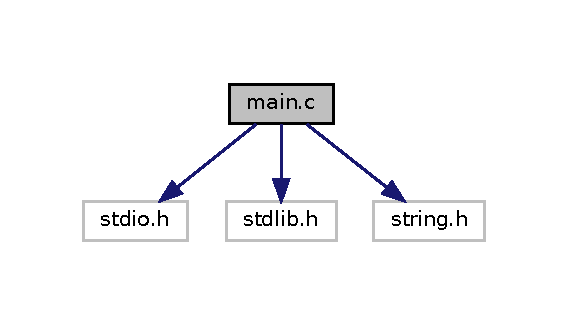
\includegraphics[width=273pt]{main_8c__incl}
\end{center}
\end{figure}
\subsection*{Functions}
\begin{DoxyCompactItemize}
\item 
int \hyperlink{main_8c_a0ddf1224851353fc92bfbff6f499fa97_a0ddf1224851353fc92bfbff6f499fa97}{main} (int argc, char $\ast$argv\mbox{[}$\,$\mbox{]})
\end{DoxyCompactItemize}


\subsection{Function Documentation}
\mbox{\Hypertarget{main_8c_a0ddf1224851353fc92bfbff6f499fa97_a0ddf1224851353fc92bfbff6f499fa97}\label{main_8c_a0ddf1224851353fc92bfbff6f499fa97_a0ddf1224851353fc92bfbff6f499fa97}} 
\index{main.\+c@{main.\+c}!main@{main}}
\index{main@{main}!main.\+c@{main.\+c}}
\subsubsection{\texorpdfstring{main()}{main()}}
{\footnotesize\ttfamily int main (\begin{DoxyParamCaption}\item[{int}]{argc,  }\item[{char $\ast$}]{argv\mbox{[}$\,$\mbox{]} }\end{DoxyParamCaption})}


\hypertarget{Misc_8h}{}\section{Misc.\+h File Reference}
\label{Misc_8h}\index{Misc.\+h@{Misc.\+h}}
{\ttfamily \#include $<$stdio.\+h$>$}\newline
{\ttfamily \#include $<$stdlib.\+h$>$}\newline
{\ttfamily \#include $<$string.\+h$>$}\newline
Include dependency graph for Misc.\+h\+:\nopagebreak
\begin{figure}[H]
\begin{center}
\leavevmode
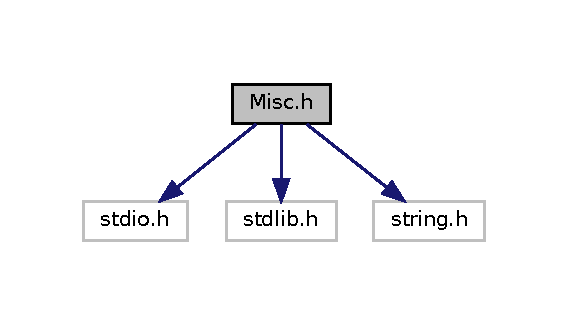
\includegraphics[width=273pt]{Misc_8h__incl}
\end{center}
\end{figure}
This graph shows which files directly or indirectly include this file\+:
\nopagebreak
\begin{figure}[H]
\begin{center}
\leavevmode
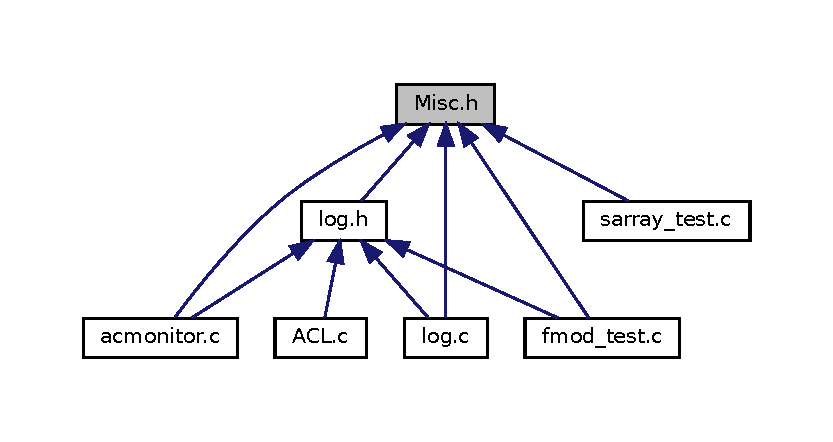
\includegraphics[width=350pt]{Misc_8h__dep__incl}
\end{center}
\end{figure}
\subsection*{Data Structures}
\begin{DoxyCompactItemize}
\item 
struct \hyperlink{structarray__1d}{array\+\_\+1d}
\begin{DoxyCompactList}\small\item\em A structure to store a 1D array of any type of data. \end{DoxyCompactList}\item 
struct \hyperlink{structString__array}{String\+\_\+array}
\begin{DoxyCompactList}\small\item\em A structure to store an array of strings. \end{DoxyCompactList}\end{DoxyCompactItemize}
\subsection*{Macros}
\begin{DoxyCompactItemize}
\item 
\#define \hyperlink{Misc_8h_ac4c027058e9ccd1d4dce6a718af0b422_ac4c027058e9ccd1d4dce6a718af0b422}{printd}(format, ...)
\item 
\#define \hyperlink{Misc_8h_a8b3a3c4c8735fffe0d3b0ab6c7053667_a8b3a3c4c8735fffe0d3b0ab6c7053667}{printld}(format, ...)
\end{DoxyCompactItemize}
\subsection*{Typedefs}
\begin{DoxyCompactItemize}
\item 
typedef struct \hyperlink{structarray__1d}{array\+\_\+1d} \hyperlink{Misc_8h_a00cef65fdcdf049cdfa42839691a9b45_a00cef65fdcdf049cdfa42839691a9b45}{array\+\_\+t}
\begin{DoxyCompactList}\small\item\em A structure to store a 1D array of any type of data. \end{DoxyCompactList}\item 
typedef struct \hyperlink{structString__array}{String\+\_\+array} \hyperlink{Misc_8h_a5415baf6b33c31bbf88da7909cacef53_a5415baf6b33c31bbf88da7909cacef53}{String\+\_\+array\+\_\+t}
\begin{DoxyCompactList}\small\item\em A structure to store an array of strings. \end{DoxyCompactList}\end{DoxyCompactItemize}
\subsection*{Functions}
\begin{DoxyCompactItemize}
\item 
\hyperlink{Misc_8h_a5415baf6b33c31bbf88da7909cacef53_a5415baf6b33c31bbf88da7909cacef53}{String\+\_\+array\+\_\+t} \hyperlink{Misc_8h_a14994f08225f3ec039c5e1c4f1ce34fe_a14994f08225f3ec039c5e1c4f1ce34fe}{Init\+String\+Array} (size\+\_\+t \+\_\+data\+\_\+size)
\item 
void \hyperlink{Misc_8h_a4dd7ace1bf25b5d9d86f09aa24eef635_a4dd7ace1bf25b5d9d86f09aa24eef635}{Push\+String\+Array} (\hyperlink{Misc_8h_a5415baf6b33c31bbf88da7909cacef53_a5415baf6b33c31bbf88da7909cacef53}{String\+\_\+array\+\_\+t} $\ast$restrict arr, const char $\ast$restrict str)
\item 
char $\ast$ \hyperlink{Misc_8h_a857fdfde68bcf52b34e778991f4f96e2_a857fdfde68bcf52b34e778991f4f96e2}{read\+String\+Array} (\hyperlink{Misc_8h_a5415baf6b33c31bbf88da7909cacef53_a5415baf6b33c31bbf88da7909cacef53}{String\+\_\+array\+\_\+t} $\ast$arr, unsigned int \+\_\+index)
\item 
int \hyperlink{Misc_8h_adf1e7a762b0fcaf97f02c286c8969b17_adf1e7a762b0fcaf97f02c286c8969b17}{set\+String\+Array} (\hyperlink{Misc_8h_a5415baf6b33c31bbf88da7909cacef53_a5415baf6b33c31bbf88da7909cacef53}{String\+\_\+array\+\_\+t} $\ast$restrict arr, unsigned int \+\_\+index, const char $\ast$restrict str)
\item 
void \hyperlink{Misc_8h_ae86e050e2e40fb2c8021bc9fd18d7672_ae86e050e2e40fb2c8021bc9fd18d7672}{Free\+String\+Array} (\hyperlink{Misc_8h_a5415baf6b33c31bbf88da7909cacef53_a5415baf6b33c31bbf88da7909cacef53}{String\+\_\+array\+\_\+t} $\ast$arr)
\end{DoxyCompactItemize}


\subsection{Macro Definition Documentation}
\mbox{\Hypertarget{Misc_8h_ac4c027058e9ccd1d4dce6a718af0b422_ac4c027058e9ccd1d4dce6a718af0b422}\label{Misc_8h_ac4c027058e9ccd1d4dce6a718af0b422_ac4c027058e9ccd1d4dce6a718af0b422}} 
\index{Misc.\+h@{Misc.\+h}!printd@{printd}}
\index{printd@{printd}!Misc.\+h@{Misc.\+h}}
\subsubsection{\texorpdfstring{printd}{printd}}
{\footnotesize\ttfamily \#define printd(\begin{DoxyParamCaption}\item[{}]{format,  }\item[{}]{... }\end{DoxyParamCaption})}

\mbox{\Hypertarget{Misc_8h_a8b3a3c4c8735fffe0d3b0ab6c7053667_a8b3a3c4c8735fffe0d3b0ab6c7053667}\label{Misc_8h_a8b3a3c4c8735fffe0d3b0ab6c7053667_a8b3a3c4c8735fffe0d3b0ab6c7053667}} 
\index{Misc.\+h@{Misc.\+h}!printld@{printld}}
\index{printld@{printld}!Misc.\+h@{Misc.\+h}}
\subsubsection{\texorpdfstring{printld}{printld}}
{\footnotesize\ttfamily \#define printld(\begin{DoxyParamCaption}\item[{}]{format,  }\item[{}]{... }\end{DoxyParamCaption})}



\subsection{Typedef Documentation}
\mbox{\Hypertarget{Misc_8h_a00cef65fdcdf049cdfa42839691a9b45_a00cef65fdcdf049cdfa42839691a9b45}\label{Misc_8h_a00cef65fdcdf049cdfa42839691a9b45_a00cef65fdcdf049cdfa42839691a9b45}} 
\index{Misc.\+h@{Misc.\+h}!array\+\_\+t@{array\+\_\+t}}
\index{array\+\_\+t@{array\+\_\+t}!Misc.\+h@{Misc.\+h}}
\subsubsection{\texorpdfstring{array\+\_\+t}{array\_t}}
{\footnotesize\ttfamily typedef struct \hyperlink{structarray__1d}{array\+\_\+1d}  \hyperlink{Misc_8h_a00cef65fdcdf049cdfa42839691a9b45_a00cef65fdcdf049cdfa42839691a9b45}{array\+\_\+t}}



A structure to store a 1D array of any type of data. 

\begin{DoxyAttention}{Attention}
The data must typecasted to void$\ast$ before storing. and must be typecasted back to the original type before using. 
\end{DoxyAttention}

\begin{DoxyParams}{Parameters}
{\em data} & A pointer to the array. \\
\hline
{\em size} & The size of the array. \\
\hline
\end{DoxyParams}
\mbox{\Hypertarget{Misc_8h_a5415baf6b33c31bbf88da7909cacef53_a5415baf6b33c31bbf88da7909cacef53}\label{Misc_8h_a5415baf6b33c31bbf88da7909cacef53_a5415baf6b33c31bbf88da7909cacef53}} 
\index{Misc.\+h@{Misc.\+h}!String\+\_\+array\+\_\+t@{String\+\_\+array\+\_\+t}}
\index{String\+\_\+array\+\_\+t@{String\+\_\+array\+\_\+t}!Misc.\+h@{Misc.\+h}}
\subsubsection{\texorpdfstring{String\+\_\+array\+\_\+t}{String\_array\_t}}
{\footnotesize\ttfamily typedef struct \hyperlink{structString__array}{String\+\_\+array}  \hyperlink{Misc_8h_a5415baf6b33c31bbf88da7909cacef53_a5415baf6b33c31bbf88da7909cacef53}{String\+\_\+array\+\_\+t}}



A structure to store an array of strings. 


\begin{DoxyParams}{Parameters}
{\em data} & A pointer to the array of strings. \\
\hline
{\em size} & The size of the array. \\
\hline
{\em capacity} & The capacity of the array. \\
\hline
{\em data\+\_\+size} & The size for each string in the array. \\
\hline
\end{DoxyParams}


\subsection{Function Documentation}
\mbox{\Hypertarget{Misc_8h_ae86e050e2e40fb2c8021bc9fd18d7672_ae86e050e2e40fb2c8021bc9fd18d7672}\label{Misc_8h_ae86e050e2e40fb2c8021bc9fd18d7672_ae86e050e2e40fb2c8021bc9fd18d7672}} 
\index{Misc.\+h@{Misc.\+h}!Free\+String\+Array@{Free\+String\+Array}}
\index{Free\+String\+Array@{Free\+String\+Array}!Misc.\+h@{Misc.\+h}}
\subsubsection{\texorpdfstring{Free\+String\+Array()}{FreeStringArray()}}
{\footnotesize\ttfamily void Free\+String\+Array (\begin{DoxyParamCaption}\item[{\hyperlink{Misc_8h_a5415baf6b33c31bbf88da7909cacef53_a5415baf6b33c31bbf88da7909cacef53}{String\+\_\+array\+\_\+t} $\ast$}]{arr }\end{DoxyParamCaption})}

\mbox{\Hypertarget{Misc_8h_a14994f08225f3ec039c5e1c4f1ce34fe_a14994f08225f3ec039c5e1c4f1ce34fe}\label{Misc_8h_a14994f08225f3ec039c5e1c4f1ce34fe_a14994f08225f3ec039c5e1c4f1ce34fe}} 
\index{Misc.\+h@{Misc.\+h}!Init\+String\+Array@{Init\+String\+Array}}
\index{Init\+String\+Array@{Init\+String\+Array}!Misc.\+h@{Misc.\+h}}
\subsubsection{\texorpdfstring{Init\+String\+Array()}{InitStringArray()}}
{\footnotesize\ttfamily \hyperlink{Misc_8h_a5415baf6b33c31bbf88da7909cacef53_a5415baf6b33c31bbf88da7909cacef53}{String\+\_\+array\+\_\+t} Init\+String\+Array (\begin{DoxyParamCaption}\item[{size\+\_\+t}]{\+\_\+data\+\_\+size }\end{DoxyParamCaption})}

\mbox{\Hypertarget{Misc_8h_a4dd7ace1bf25b5d9d86f09aa24eef635_a4dd7ace1bf25b5d9d86f09aa24eef635}\label{Misc_8h_a4dd7ace1bf25b5d9d86f09aa24eef635_a4dd7ace1bf25b5d9d86f09aa24eef635}} 
\index{Misc.\+h@{Misc.\+h}!Push\+String\+Array@{Push\+String\+Array}}
\index{Push\+String\+Array@{Push\+String\+Array}!Misc.\+h@{Misc.\+h}}
\subsubsection{\texorpdfstring{Push\+String\+Array()}{PushStringArray()}}
{\footnotesize\ttfamily void Push\+String\+Array (\begin{DoxyParamCaption}\item[{\hyperlink{Misc_8h_a5415baf6b33c31bbf88da7909cacef53_a5415baf6b33c31bbf88da7909cacef53}{String\+\_\+array\+\_\+t} $\ast$restrict}]{arr,  }\item[{const char $\ast$restrict}]{str }\end{DoxyParamCaption})}

\mbox{\Hypertarget{Misc_8h_a857fdfde68bcf52b34e778991f4f96e2_a857fdfde68bcf52b34e778991f4f96e2}\label{Misc_8h_a857fdfde68bcf52b34e778991f4f96e2_a857fdfde68bcf52b34e778991f4f96e2}} 
\index{Misc.\+h@{Misc.\+h}!read\+String\+Array@{read\+String\+Array}}
\index{read\+String\+Array@{read\+String\+Array}!Misc.\+h@{Misc.\+h}}
\subsubsection{\texorpdfstring{read\+String\+Array()}{readStringArray()}}
{\footnotesize\ttfamily char$\ast$ read\+String\+Array (\begin{DoxyParamCaption}\item[{\hyperlink{Misc_8h_a5415baf6b33c31bbf88da7909cacef53_a5415baf6b33c31bbf88da7909cacef53}{String\+\_\+array\+\_\+t} $\ast$}]{arr,  }\item[{unsigned int}]{\+\_\+index }\end{DoxyParamCaption})}

\mbox{\Hypertarget{Misc_8h_adf1e7a762b0fcaf97f02c286c8969b17_adf1e7a762b0fcaf97f02c286c8969b17}\label{Misc_8h_adf1e7a762b0fcaf97f02c286c8969b17_adf1e7a762b0fcaf97f02c286c8969b17}} 
\index{Misc.\+h@{Misc.\+h}!set\+String\+Array@{set\+String\+Array}}
\index{set\+String\+Array@{set\+String\+Array}!Misc.\+h@{Misc.\+h}}
\subsubsection{\texorpdfstring{set\+String\+Array()}{setStringArray()}}
{\footnotesize\ttfamily int set\+String\+Array (\begin{DoxyParamCaption}\item[{\hyperlink{Misc_8h_a5415baf6b33c31bbf88da7909cacef53_a5415baf6b33c31bbf88da7909cacef53}{String\+\_\+array\+\_\+t} $\ast$restrict}]{arr,  }\item[{unsigned int}]{\+\_\+index,  }\item[{const char $\ast$restrict}]{str }\end{DoxyParamCaption})}


\hypertarget{README_8md}{}\section{R\+E\+A\+D\+M\+E.\+md File Reference}
\label{README_8md}\index{R\+E\+A\+D\+M\+E.\+md@{R\+E\+A\+D\+M\+E.\+md}}

\hypertarget{sarray__test_8c}{}\section{sarray\+\_\+test.\+c File Reference}
\label{sarray__test_8c}\index{sarray\+\_\+test.\+c@{sarray\+\_\+test.\+c}}
{\ttfamily \#include \char`\"{}../lib/\+Misc.\+h\char`\"{}}\newline
Include dependency graph for sarray\+\_\+test.\+c\+:
\nopagebreak
\begin{figure}[H]
\begin{center}
\leavevmode
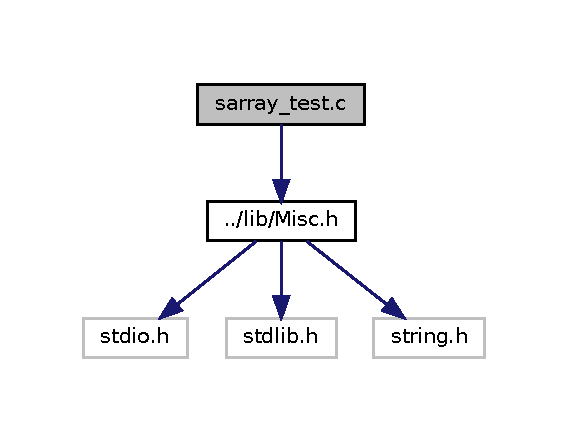
\includegraphics[width=273pt]{sarray__test_8c__incl}
\end{center}
\end{figure}
\subsection*{Macros}
\begin{DoxyCompactItemize}
\item 
\#define \hyperlink{sarray__test_8c_a8d23feea868a983c8c2b661e1e16972f_a8d23feea868a983c8c2b661e1e16972f}{R\+ED}~\char`\"{}\textbackslash{}x1B\mbox{[}31m\char`\"{}
\item 
\#define \hyperlink{sarray__test_8c_aea69ffbacdcdf16c21b8c9961df84448_aea69ffbacdcdf16c21b8c9961df84448}{G\+RN}~\char`\"{}\textbackslash{}x1B\mbox{[}32m\char`\"{}
\item 
\#define \hyperlink{sarray__test_8c_a96fac03c4ab3363f06a0328e0e53a40c_a96fac03c4ab3363f06a0328e0e53a40c}{Y\+EL}~\char`\"{}\textbackslash{}x1B\mbox{[}33m\char`\"{}
\item 
\#define \hyperlink{sarray__test_8c_add9307de87f38e77d336751e305886f6_add9307de87f38e77d336751e305886f6}{B\+LU}~\char`\"{}\textbackslash{}x1B\mbox{[}34m\char`\"{}
\item 
\#define \hyperlink{sarray__test_8c_af54a5a977c0c499323d656315f008ee0_af54a5a977c0c499323d656315f008ee0}{M\+AG}~\char`\"{}\textbackslash{}x1B\mbox{[}35m\char`\"{}
\item 
\#define \hyperlink{sarray__test_8c_adc708fa688f5d78db361f66c36f0f807_adc708fa688f5d78db361f66c36f0f807}{C\+YN}~\char`\"{}\textbackslash{}x1B\mbox{[}36m\char`\"{}
\item 
\#define \hyperlink{sarray__test_8c_aeaf3a04d5bf63b204689a714718ea930_aeaf3a04d5bf63b204689a714718ea930}{W\+HT}~\char`\"{}\textbackslash{}x1B\mbox{[}37m\char`\"{}
\item 
\#define \hyperlink{sarray__test_8c_ab702106cf3b3e96750b6845ded4e0299_ab702106cf3b3e96750b6845ded4e0299}{R\+E\+S\+ET}~\char`\"{}\textbackslash{}x1B\mbox{[}0m\char`\"{}
\item 
\#define \hyperlink{sarray__test_8c_a067c26d9816bdb37329ec04da22a5f66_a067c26d9816bdb37329ec04da22a5f66}{assert}(cond,  message)~if (!(cond)) \{ printf(\hyperlink{sarray__test_8c_a8d23feea868a983c8c2b661e1e16972f_a8d23feea868a983c8c2b661e1e16972f}{R\+ED} \char`\"{}F\+A\+I\+L\+ED\char`\"{} R\+E\+S\+ET); printf(\char`\"{}\textbackslash{}t \%s\textbackslash{}n\char`\"{}, message); return 0; \}
\end{DoxyCompactItemize}
\subsection*{Functions}
\begin{DoxyCompactItemize}
\item 
int \hyperlink{sarray__test_8c_a33f4380cb9acb2659b0a905e8f592207_a33f4380cb9acb2659b0a905e8f592207}{single\+\_\+append\+\_\+test\+\_\+} ()
\item 
int \hyperlink{sarray__test_8c_a081b7e48daa6ee1b3ee12843ecb33022_a081b7e48daa6ee1b3ee12843ecb33022}{whole\+\_\+append\+\_\+test} ()
\item 
int \hyperlink{sarray__test_8c_a0ec585a81268a550f110094062a3bb21_a0ec585a81268a550f110094062a3bb21}{single\+\_\+set\+\_\+test} ()
\item 
int \hyperlink{sarray__test_8c_a58a408c44d40525d202f3db85b83506f_a58a408c44d40525d202f3db85b83506f}{whole\+\_\+set\+\_\+test} ()
\item 
int \hyperlink{sarray__test_8c_a9dfb196b1ebe13838bd73446a407155c_a9dfb196b1ebe13838bd73446a407155c}{free\+\_\+test} ()
\item 
int \hyperlink{sarray__test_8c_ae66f6b31b5ad750f1fe042a706a4e3d4_ae66f6b31b5ad750f1fe042a706a4e3d4}{main} ()
\end{DoxyCompactItemize}
\subsection*{Variables}
\begin{DoxyCompactItemize}
\item 
const char $\ast$ \hyperlink{sarray__test_8c_ab834f53bdb8b437f1df34c9ed6ccf688_ab834f53bdb8b437f1df34c9ed6ccf688}{lines} \mbox{[}$\,$\mbox{]}
\item 
\hyperlink{Misc_8h_a5415baf6b33c31bbf88da7909cacef53_a5415baf6b33c31bbf88da7909cacef53}{String\+\_\+array\+\_\+t} \hyperlink{sarray__test_8c_a54b7719ced86bec3a7f9f94be2cc7fa0_a54b7719ced86bec3a7f9f94be2cc7fa0}{U\+UT}
\end{DoxyCompactItemize}


\subsection{Macro Definition Documentation}
\mbox{\Hypertarget{sarray__test_8c_a067c26d9816bdb37329ec04da22a5f66_a067c26d9816bdb37329ec04da22a5f66}\label{sarray__test_8c_a067c26d9816bdb37329ec04da22a5f66_a067c26d9816bdb37329ec04da22a5f66}} 
\index{sarray\+\_\+test.\+c@{sarray\+\_\+test.\+c}!assert@{assert}}
\index{assert@{assert}!sarray\+\_\+test.\+c@{sarray\+\_\+test.\+c}}
\subsubsection{\texorpdfstring{assert}{assert}}
{\footnotesize\ttfamily \#define assert(\begin{DoxyParamCaption}\item[{}]{cond,  }\item[{}]{message }\end{DoxyParamCaption})~if (!(cond)) \{ printf(\hyperlink{sarray__test_8c_a8d23feea868a983c8c2b661e1e16972f_a8d23feea868a983c8c2b661e1e16972f}{R\+ED} \char`\"{}F\+A\+I\+L\+ED\char`\"{} R\+E\+S\+ET); printf(\char`\"{}\textbackslash{}t \%s\textbackslash{}n\char`\"{}, message); return 0; \}}

\mbox{\Hypertarget{sarray__test_8c_add9307de87f38e77d336751e305886f6_add9307de87f38e77d336751e305886f6}\label{sarray__test_8c_add9307de87f38e77d336751e305886f6_add9307de87f38e77d336751e305886f6}} 
\index{sarray\+\_\+test.\+c@{sarray\+\_\+test.\+c}!B\+LU@{B\+LU}}
\index{B\+LU@{B\+LU}!sarray\+\_\+test.\+c@{sarray\+\_\+test.\+c}}
\subsubsection{\texorpdfstring{B\+LU}{BLU}}
{\footnotesize\ttfamily \#define B\+LU~\char`\"{}\textbackslash{}x1B\mbox{[}34m\char`\"{}}

\mbox{\Hypertarget{sarray__test_8c_adc708fa688f5d78db361f66c36f0f807_adc708fa688f5d78db361f66c36f0f807}\label{sarray__test_8c_adc708fa688f5d78db361f66c36f0f807_adc708fa688f5d78db361f66c36f0f807}} 
\index{sarray\+\_\+test.\+c@{sarray\+\_\+test.\+c}!C\+YN@{C\+YN}}
\index{C\+YN@{C\+YN}!sarray\+\_\+test.\+c@{sarray\+\_\+test.\+c}}
\subsubsection{\texorpdfstring{C\+YN}{CYN}}
{\footnotesize\ttfamily \#define C\+YN~\char`\"{}\textbackslash{}x1B\mbox{[}36m\char`\"{}}

\mbox{\Hypertarget{sarray__test_8c_aea69ffbacdcdf16c21b8c9961df84448_aea69ffbacdcdf16c21b8c9961df84448}\label{sarray__test_8c_aea69ffbacdcdf16c21b8c9961df84448_aea69ffbacdcdf16c21b8c9961df84448}} 
\index{sarray\+\_\+test.\+c@{sarray\+\_\+test.\+c}!G\+RN@{G\+RN}}
\index{G\+RN@{G\+RN}!sarray\+\_\+test.\+c@{sarray\+\_\+test.\+c}}
\subsubsection{\texorpdfstring{G\+RN}{GRN}}
{\footnotesize\ttfamily \#define G\+RN~\char`\"{}\textbackslash{}x1B\mbox{[}32m\char`\"{}}

\mbox{\Hypertarget{sarray__test_8c_af54a5a977c0c499323d656315f008ee0_af54a5a977c0c499323d656315f008ee0}\label{sarray__test_8c_af54a5a977c0c499323d656315f008ee0_af54a5a977c0c499323d656315f008ee0}} 
\index{sarray\+\_\+test.\+c@{sarray\+\_\+test.\+c}!M\+AG@{M\+AG}}
\index{M\+AG@{M\+AG}!sarray\+\_\+test.\+c@{sarray\+\_\+test.\+c}}
\subsubsection{\texorpdfstring{M\+AG}{MAG}}
{\footnotesize\ttfamily \#define M\+AG~\char`\"{}\textbackslash{}x1B\mbox{[}35m\char`\"{}}

\mbox{\Hypertarget{sarray__test_8c_a8d23feea868a983c8c2b661e1e16972f_a8d23feea868a983c8c2b661e1e16972f}\label{sarray__test_8c_a8d23feea868a983c8c2b661e1e16972f_a8d23feea868a983c8c2b661e1e16972f}} 
\index{sarray\+\_\+test.\+c@{sarray\+\_\+test.\+c}!R\+ED@{R\+ED}}
\index{R\+ED@{R\+ED}!sarray\+\_\+test.\+c@{sarray\+\_\+test.\+c}}
\subsubsection{\texorpdfstring{R\+ED}{RED}}
{\footnotesize\ttfamily \#define R\+ED~\char`\"{}\textbackslash{}x1B\mbox{[}31m\char`\"{}}

\mbox{\Hypertarget{sarray__test_8c_ab702106cf3b3e96750b6845ded4e0299_ab702106cf3b3e96750b6845ded4e0299}\label{sarray__test_8c_ab702106cf3b3e96750b6845ded4e0299_ab702106cf3b3e96750b6845ded4e0299}} 
\index{sarray\+\_\+test.\+c@{sarray\+\_\+test.\+c}!R\+E\+S\+ET@{R\+E\+S\+ET}}
\index{R\+E\+S\+ET@{R\+E\+S\+ET}!sarray\+\_\+test.\+c@{sarray\+\_\+test.\+c}}
\subsubsection{\texorpdfstring{R\+E\+S\+ET}{RESET}}
{\footnotesize\ttfamily \#define R\+E\+S\+ET~\char`\"{}\textbackslash{}x1B\mbox{[}0m\char`\"{}}

\mbox{\Hypertarget{sarray__test_8c_aeaf3a04d5bf63b204689a714718ea930_aeaf3a04d5bf63b204689a714718ea930}\label{sarray__test_8c_aeaf3a04d5bf63b204689a714718ea930_aeaf3a04d5bf63b204689a714718ea930}} 
\index{sarray\+\_\+test.\+c@{sarray\+\_\+test.\+c}!W\+HT@{W\+HT}}
\index{W\+HT@{W\+HT}!sarray\+\_\+test.\+c@{sarray\+\_\+test.\+c}}
\subsubsection{\texorpdfstring{W\+HT}{WHT}}
{\footnotesize\ttfamily \#define W\+HT~\char`\"{}\textbackslash{}x1B\mbox{[}37m\char`\"{}}

\mbox{\Hypertarget{sarray__test_8c_a96fac03c4ab3363f06a0328e0e53a40c_a96fac03c4ab3363f06a0328e0e53a40c}\label{sarray__test_8c_a96fac03c4ab3363f06a0328e0e53a40c_a96fac03c4ab3363f06a0328e0e53a40c}} 
\index{sarray\+\_\+test.\+c@{sarray\+\_\+test.\+c}!Y\+EL@{Y\+EL}}
\index{Y\+EL@{Y\+EL}!sarray\+\_\+test.\+c@{sarray\+\_\+test.\+c}}
\subsubsection{\texorpdfstring{Y\+EL}{YEL}}
{\footnotesize\ttfamily \#define Y\+EL~\char`\"{}\textbackslash{}x1B\mbox{[}33m\char`\"{}}



\subsection{Function Documentation}
\mbox{\Hypertarget{sarray__test_8c_a9dfb196b1ebe13838bd73446a407155c_a9dfb196b1ebe13838bd73446a407155c}\label{sarray__test_8c_a9dfb196b1ebe13838bd73446a407155c_a9dfb196b1ebe13838bd73446a407155c}} 
\index{sarray\+\_\+test.\+c@{sarray\+\_\+test.\+c}!free\+\_\+test@{free\+\_\+test}}
\index{free\+\_\+test@{free\+\_\+test}!sarray\+\_\+test.\+c@{sarray\+\_\+test.\+c}}
\subsubsection{\texorpdfstring{free\+\_\+test()}{free\_test()}}
{\footnotesize\ttfamily int free\+\_\+test (\begin{DoxyParamCaption}{ }\end{DoxyParamCaption})}

\begin{DoxyRefDesc}{Test}
\item[\hyperlink{test__test000005}{Test}]Test the free function of \hyperlink{}{Misk.\+h}. \end{DoxyRefDesc}
\mbox{\Hypertarget{sarray__test_8c_ae66f6b31b5ad750f1fe042a706a4e3d4_ae66f6b31b5ad750f1fe042a706a4e3d4}\label{sarray__test_8c_ae66f6b31b5ad750f1fe042a706a4e3d4_ae66f6b31b5ad750f1fe042a706a4e3d4}} 
\index{sarray\+\_\+test.\+c@{sarray\+\_\+test.\+c}!main@{main}}
\index{main@{main}!sarray\+\_\+test.\+c@{sarray\+\_\+test.\+c}}
\subsubsection{\texorpdfstring{main()}{main()}}
{\footnotesize\ttfamily int main (\begin{DoxyParamCaption}\item[{void}]{ }\end{DoxyParamCaption})}

\mbox{\Hypertarget{sarray__test_8c_a33f4380cb9acb2659b0a905e8f592207_a33f4380cb9acb2659b0a905e8f592207}\label{sarray__test_8c_a33f4380cb9acb2659b0a905e8f592207_a33f4380cb9acb2659b0a905e8f592207}} 
\index{sarray\+\_\+test.\+c@{sarray\+\_\+test.\+c}!single\+\_\+append\+\_\+test\+\_\+@{single\+\_\+append\+\_\+test\+\_\+}}
\index{single\+\_\+append\+\_\+test\+\_\+@{single\+\_\+append\+\_\+test\+\_\+}!sarray\+\_\+test.\+c@{sarray\+\_\+test.\+c}}
\subsubsection{\texorpdfstring{single\+\_\+append\+\_\+test\+\_\+()}{single\_append\_test\_()}}
{\footnotesize\ttfamily int single\+\_\+append\+\_\+test\+\_\+ (\begin{DoxyParamCaption}{ }\end{DoxyParamCaption})}

\begin{DoxyRefDesc}{Test}
\item[\hyperlink{test__test000001}{Test}]Test the append function of \hyperlink{}{Misk.\+h}. \end{DoxyRefDesc}
\mbox{\Hypertarget{sarray__test_8c_a0ec585a81268a550f110094062a3bb21_a0ec585a81268a550f110094062a3bb21}\label{sarray__test_8c_a0ec585a81268a550f110094062a3bb21_a0ec585a81268a550f110094062a3bb21}} 
\index{sarray\+\_\+test.\+c@{sarray\+\_\+test.\+c}!single\+\_\+set\+\_\+test@{single\+\_\+set\+\_\+test}}
\index{single\+\_\+set\+\_\+test@{single\+\_\+set\+\_\+test}!sarray\+\_\+test.\+c@{sarray\+\_\+test.\+c}}
\subsubsection{\texorpdfstring{single\+\_\+set\+\_\+test()}{single\_set\_test()}}
{\footnotesize\ttfamily int single\+\_\+set\+\_\+test (\begin{DoxyParamCaption}{ }\end{DoxyParamCaption})}

\begin{DoxyRefDesc}{Test}
\item[\hyperlink{test__test000003}{Test}]Test the set function of \hyperlink{}{Misk.\+h}. \end{DoxyRefDesc}
\mbox{\Hypertarget{sarray__test_8c_a081b7e48daa6ee1b3ee12843ecb33022_a081b7e48daa6ee1b3ee12843ecb33022}\label{sarray__test_8c_a081b7e48daa6ee1b3ee12843ecb33022_a081b7e48daa6ee1b3ee12843ecb33022}} 
\index{sarray\+\_\+test.\+c@{sarray\+\_\+test.\+c}!whole\+\_\+append\+\_\+test@{whole\+\_\+append\+\_\+test}}
\index{whole\+\_\+append\+\_\+test@{whole\+\_\+append\+\_\+test}!sarray\+\_\+test.\+c@{sarray\+\_\+test.\+c}}
\subsubsection{\texorpdfstring{whole\+\_\+append\+\_\+test()}{whole\_append\_test()}}
{\footnotesize\ttfamily int whole\+\_\+append\+\_\+test (\begin{DoxyParamCaption}{ }\end{DoxyParamCaption})}

\begin{DoxyRefDesc}{Test}
\item[\hyperlink{test__test000002}{Test}]Test the append function of \hyperlink{}{Misk.\+h}. \end{DoxyRefDesc}
\mbox{\Hypertarget{sarray__test_8c_a58a408c44d40525d202f3db85b83506f_a58a408c44d40525d202f3db85b83506f}\label{sarray__test_8c_a58a408c44d40525d202f3db85b83506f_a58a408c44d40525d202f3db85b83506f}} 
\index{sarray\+\_\+test.\+c@{sarray\+\_\+test.\+c}!whole\+\_\+set\+\_\+test@{whole\+\_\+set\+\_\+test}}
\index{whole\+\_\+set\+\_\+test@{whole\+\_\+set\+\_\+test}!sarray\+\_\+test.\+c@{sarray\+\_\+test.\+c}}
\subsubsection{\texorpdfstring{whole\+\_\+set\+\_\+test()}{whole\_set\_test()}}
{\footnotesize\ttfamily int whole\+\_\+set\+\_\+test (\begin{DoxyParamCaption}{ }\end{DoxyParamCaption})}

\begin{DoxyRefDesc}{Test}
\item[\hyperlink{test__test000004}{Test}]Test the set function of \hyperlink{}{Misk.\+h}. \end{DoxyRefDesc}


\subsection{Variable Documentation}
\mbox{\Hypertarget{sarray__test_8c_ab834f53bdb8b437f1df34c9ed6ccf688_ab834f53bdb8b437f1df34c9ed6ccf688}\label{sarray__test_8c_ab834f53bdb8b437f1df34c9ed6ccf688_ab834f53bdb8b437f1df34c9ed6ccf688}} 
\index{sarray\+\_\+test.\+c@{sarray\+\_\+test.\+c}!lines@{lines}}
\index{lines@{lines}!sarray\+\_\+test.\+c@{sarray\+\_\+test.\+c}}
\subsubsection{\texorpdfstring{lines}{lines}}
{\footnotesize\ttfamily const char$\ast$ lines\mbox{[}$\,$\mbox{]}}

{\bfseries Initial value\+:}
\begin{DoxyCode}
= \{
    \textcolor{stringliteral}{"And disciplinary remains mercifully"},
    \textcolor{stringliteral}{"Yes and um, I'm with you Derek, this star nonsense"},
    \textcolor{stringliteral}{"Yes, yes"},
    \textcolor{stringliteral}{"Now which is it?"},
    \textcolor{stringliteral}{"I am sure of it"},
    \textcolor{stringliteral}{"So, so you think you can tell"},
    \textcolor{stringliteral}{"Heaven from hell?"},
    \textcolor{stringliteral}{"Blue skies from pain?"},
    \textcolor{stringliteral}{"Can you tell a green field"},
    \textcolor{stringliteral}{"From a cold steel rail?"},
    \textcolor{stringliteral}{"A smile from a veil?"},
    \textcolor{stringliteral}{"Do you think you can tell?"},
    \textcolor{stringliteral}{"Did they get you to trade"},
    \textcolor{stringliteral}{"Your heroes for ghosts?"},
    \textcolor{stringliteral}{"Hot ashes for trees?"},
    \textcolor{stringliteral}{"Hot air for a cool breeze?"},
    \textcolor{stringliteral}{"Cold comfort for change?"},
    \textcolor{stringliteral}{"Did you exchange"},
    \textcolor{stringliteral}{"A walk-on part in the war"},
    \textcolor{stringliteral}{"For a lead role in a cage?"},
    \textcolor{stringliteral}{"How I wish, how I wish you were here"},
    \textcolor{stringliteral}{"We're just two lost souls"},
    \textcolor{stringliteral}{"Swimming in a fish bowl"},
    \textcolor{stringliteral}{"Year after year"},
    \textcolor{stringliteral}{"Running over the same old ground"},
    \textcolor{stringliteral}{"What have we found?"},
    \textcolor{stringliteral}{"The same old fears"},
    \textcolor{stringliteral}{"Wish you were here"}
\}
\end{DoxyCode}
\mbox{\Hypertarget{sarray__test_8c_a54b7719ced86bec3a7f9f94be2cc7fa0_a54b7719ced86bec3a7f9f94be2cc7fa0}\label{sarray__test_8c_a54b7719ced86bec3a7f9f94be2cc7fa0_a54b7719ced86bec3a7f9f94be2cc7fa0}} 
\index{sarray\+\_\+test.\+c@{sarray\+\_\+test.\+c}!U\+UT@{U\+UT}}
\index{U\+UT@{U\+UT}!sarray\+\_\+test.\+c@{sarray\+\_\+test.\+c}}
\subsubsection{\texorpdfstring{U\+UT}{UUT}}
{\footnotesize\ttfamily \hyperlink{Misc_8h_a5415baf6b33c31bbf88da7909cacef53_a5415baf6b33c31bbf88da7909cacef53}{String\+\_\+array\+\_\+t} U\+UT}


\hypertarget{template_8c}{}\section{template.\+c File Reference}
\label{template_8c}\index{template.\+c@{template.\+c}}
{\ttfamily \#include $<$stdio.\+h$>$}\newline
Include dependency graph for template.\+c\+:
\nopagebreak
\begin{figure}[H]
\begin{center}
\leavevmode
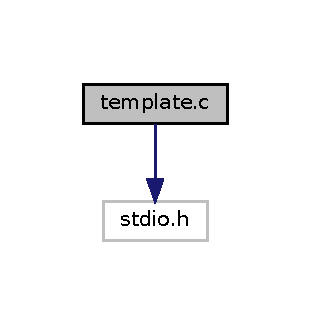
\includegraphics[width=149pt]{template_8c__incl}
\end{center}
\end{figure}
\subsection*{Functions}
\begin{DoxyCompactItemize}
\item 
int \hyperlink{template_8c_a0ddf1224851353fc92bfbff6f499fa97_a0ddf1224851353fc92bfbff6f499fa97}{main} (int argc, char $\ast$argv\mbox{[}$\,$\mbox{]})
\end{DoxyCompactItemize}


\subsection{Function Documentation}
\mbox{\Hypertarget{template_8c_a0ddf1224851353fc92bfbff6f499fa97_a0ddf1224851353fc92bfbff6f499fa97}\label{template_8c_a0ddf1224851353fc92bfbff6f499fa97_a0ddf1224851353fc92bfbff6f499fa97}} 
\index{template.\+c@{template.\+c}!main@{main}}
\index{main@{main}!template.\+c@{template.\+c}}
\subsubsection{\texorpdfstring{main()}{main()}}
{\footnotesize\ttfamily int main (\begin{DoxyParamCaption}\item[{int}]{argc,  }\item[{char $\ast$}]{argv\mbox{[}$\,$\mbox{]} }\end{DoxyParamCaption})}


\hypertarget{test__aclog_8c}{}\section{test\+\_\+aclog.\+c File Reference}
\label{test__aclog_8c}\index{test\+\_\+aclog.\+c@{test\+\_\+aclog.\+c}}
{\ttfamily \#include $<$stdio.\+h$>$}\newline
{\ttfamily \#include $<$stdlib.\+h$>$}\newline
Include dependency graph for test\+\_\+aclog.\+c\+:
\nopagebreak
\begin{figure}[H]
\begin{center}
\leavevmode
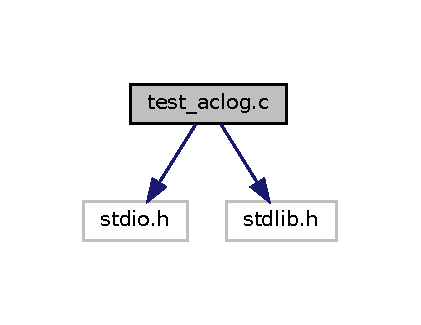
\includegraphics[width=202pt]{test__aclog_8c__incl}
\end{center}
\end{figure}
\subsection*{Functions}
\begin{DoxyCompactItemize}
\item 
int \hyperlink{test__aclog_8c_ae66f6b31b5ad750f1fe042a706a4e3d4_ae66f6b31b5ad750f1fe042a706a4e3d4}{main} ()
\end{DoxyCompactItemize}


\subsection{Function Documentation}
\mbox{\Hypertarget{test__aclog_8c_ae66f6b31b5ad750f1fe042a706a4e3d4_ae66f6b31b5ad750f1fe042a706a4e3d4}\label{test__aclog_8c_ae66f6b31b5ad750f1fe042a706a4e3d4_ae66f6b31b5ad750f1fe042a706a4e3d4}} 
\index{test\+\_\+aclog.\+c@{test\+\_\+aclog.\+c}!main@{main}}
\index{main@{main}!test\+\_\+aclog.\+c@{test\+\_\+aclog.\+c}}
\subsubsection{\texorpdfstring{main()}{main()}}
{\footnotesize\ttfamily int main (\begin{DoxyParamCaption}\item[{void}]{ }\end{DoxyParamCaption})}


\chapter{Example Documentation}
\hypertarget{char-example}{}\section{char}
read a string from the string array. $\ast$str = read\+String\+Array(\&arr, 0); 
\begin{DoxyParams}{Parameters}
{\em arr} & A pointer to the string array. \\
\hline
{\em \+\_\+index} & The index of the string to be read.\\
\hline
\end{DoxyParams}
\begin{DoxyReturn}{Returns}
char$\ast$ returns the sting pointed to by the \hyperlink{}{\+\_\+index}.
\end{DoxyReturn}

\begin{DoxyCodeInclude}
\end{DoxyCodeInclude}
 
\hypertarget{FreeStringArray-example}{}\section{Free\+String\+Array}
Free the string array. (\&arr); 
\begin{DoxyParams}{Parameters}
{\em arr} & A pointer to the string array.\\
\hline
\end{DoxyParams}

\begin{DoxyCodeInclude}
\end{DoxyCodeInclude}
 
\hypertarget{gcc-example}{}\section{gcc}
\begin{DoxyVersion}{Version}
1.\+1.\+3 
\end{DoxyVersion}
\begin{DoxyAuthor}{Authors}
mkritikakis, hgeorgakopoulos
\end{DoxyAuthor}
This file contains the functions to create and print log entries onto log.\+txt Hooks for fopen, fread, fwrite and fclose are present and can be enabled by defining the macros \+\_\+\+\_\+\+H\+O\+P\+EN, \+\_\+\+\_\+\+H\+R\+E\+AD, \+\_\+\+\_\+\+H\+W\+R\+I\+TE and \+\_\+\+\_\+\+H\+D\+E\+L\+E\+TE respectively. -\/\+D\+\_\+\+\_\+\+H\+O\+P\+EN -\/\+D\+\_\+\+\_\+\+H\+R\+E\+AD -\/\+D\+\_\+\+\_\+\+H\+W\+R\+I\+TE -\/\+D\+\_\+\+\_\+\+H\+D\+E\+L\+E\+TE -\/o test test.\+c \hyperlink{ACL_8c}{lib/\+A\+C\+L.\+c} \hyperlink{log_8c}{lib/log.\+c} \hyperlink{fhandler_8c}{lib/fhandler.\+c}

This file is compiled into a shared object file and is loaded into the process address space of the target program using L\+D\+\_\+\+P\+R\+E\+L\+O\+AD.


\begin{DoxyCodeInclude}
\end{DoxyCodeInclude}
 
\hypertarget{LD_PRELOAD-example}{}\section{L\+D\+\_\+\+P\+R\+E\+L\+O\+AD}
=./lib\+A\+CL.so $<$executable$>$

This file can be preloaded into the system with the following command. This way each file access will be logged.


\begin{DoxyCodeInclude}
\end{DoxyCodeInclude}
 
\hypertarget{PushStringArray-example}{}\section{Push\+String\+Array}
Push a string to the string array. (\&arr, \char`\"{}\+Hello World\char`\"{}); 
\begin{DoxyParams}{Parameters}
{\em arr} & A pointer to the string array. \\
\hline
{\em str} & The string to be pushed. \\
\hline
\end{DoxyParams}
\begin{DoxyReturn}{Returns}
void
\end{DoxyReturn}
\begin{DoxyRefDesc}{Todo}
\item[\hyperlink{todo__todo000003}{Todo}]Add a check for the size of the string. 

return an error code. \end{DoxyRefDesc}



\begin{DoxyCodeInclude}
\end{DoxyCodeInclude}
 
\hypertarget{setStringArray-example}{}\section{set\+String\+Array}
Set a string in the string array. (\&arr, 0, \char`\"{}\+Hello World\char`\"{}); 
\begin{DoxyParams}{Parameters}
{\em arr} & A pointer to the string array. \\
\hline
{\em \+\_\+index} & The index to the string to be set. \\
\hline
{\em str} & The string to be set.\\
\hline
\end{DoxyParams}
\begin{DoxyReturn}{Returns}
int returns -\/1 when \hyperlink{}{\+\_\+index} is larger than the \hyperlink{}{\+\_\+size}. returns 1 on success.
\end{DoxyReturn}

\begin{DoxyCodeInclude}
\end{DoxyCodeInclude}
 
\hypertarget{String_array_t-example}{}\section{String\+\_\+array\+\_\+t}
Initialize a the string array. arr = Init\+String\+Array(256); 
\begin{DoxyParams}{Parameters}
{\em \+\_\+data\+\_\+size} & The size for each string in the array. \\
\hline
\end{DoxyParams}
\begin{DoxyReturn}{Returns}
String\+\_\+array\+\_\+t
\end{DoxyReturn}

\begin{DoxyCodeInclude}
\end{DoxyCodeInclude}
 
%--- End generated contents ---

% Index
\backmatter
\newpage
\phantomsection
\clearemptydoublepage
\addcontentsline{toc}{chapter}{Index}
\printindex

\end{document}
